\documentclass[11pt]{article}
\usepackage{amsmath}
\usepackage{amssymb}
\usepackage{epic,gastex}
\usepackage{array}
\usepackage{graphicx}

\usepackage[utf8]{inputenc}
\usepackage[russian]{babel}


\newcommand{\sa}{synchronizing automata}
\newcommand{\san}{synchronizing automaton}
\newcommand{\sw}{reset word}
\newcommand{\sws}{reset words}
\newcommand{\ssw}{reset word of minimum length}
\newcommand{\rl}{reset length}

\DeclareMathOperator{\weight}{wg}

\DeclareSymbolFont{rsfscript}{OMS}{rsfs}{m}{n}
\DeclareSymbolFontAlphabet{\mathrsfs}{rsfscript}

\newtheorem{theorem}{Утверждение}
\newtheorem{conjecture}{Гипотеза}
\newtheorem{lemma}{Лемма}

%\newcommand{\proof}{{\it Доказательство:\ }}
\newenvironment{proof}{Доказательство:}{$\square$}

\begin{document}
\title{Медленно-синхронизируемые автоматы и ориентированные графы\thanks{Работа выполнена
при финансовой поддержке Российского фонда фундаментальных исследований(гранты 09-01-12142
и 10-01-00524), а также при поддержке Федерального агентства по образованию (грант 2.1.1/3537).}}

%\titlerunning{Медленно-синхронизируемые автоматы и ориентированные графы}

%\author{D. S. Ananichev \and V. V. Gusev \and M. V. Volkov}

%\authorrunning{D. S. Ananichev, V. V. Gusev, M. V. Volkov}

%\tocauthor{D. S. Ananichev, V. V. Gusev, M. V. Volkov (Ekaterinburg, Russia)}

%\institute{Department of Mathematics and Mechanics,\\
%Ural State University, 620083 Ekaterinburg, RUSSIA\\
%\email{Dmitry.Ananichev@usu.ru, vl.gusev@gmail.com,
%Mikhail.Volkov@usu.ru}}

\maketitle


\begin{abstract}
Мы приводим несколько бесконечных серий синхронизируемых автоматов, 
длина кратчайшего синхронизирующего слова которых близка к квадрату числа состояний.
Эти автоматы тесно связаны с примитивными ориентированными графами
с большой экспонентой.
\end{abstract}


%
%\begin{abstract}
%We present several infinite series of \sa\ for which
%the minimum length of reset words is close to the
%square of the number of states. These automata are
%closely related to primitive digraphs with large exponent.
%\end{abstract}


%\section{Background and overview}
%\label{intro}

\section{Введение}
\label{intro}

\emph{Полным детерминированным конечным автоматом} (ДКА) называется
тройка $\mathrsfs{A}=\langle Q,\Sigma,\delta\rangle$, где $Q$ и
$\Sigma$ являются конечными множествами. Множество $Q$ будем называть \emph{множеством состояний},
а $\Sigma$ \emph{входным алфавитом}. Всюду определенная функция $\delta:Q\times\Sigma\to Q$ 
называется \emph{функцией переходов}. 
Обозначим через $\Sigma^*$ множество всех конечных слов над
алфавитом $\Sigma$, включая пустое.
Функцию $\delta$ можно продолжить до функции $Q\times\Sigma^*\to Q$
(также обозначаемой $\delta$) следующим естественным образом: для
$q\in Q$ и $w\in\Sigma^*$ положим $\delta(q,w)=q$, если $w$ пусто, и 
$\delta(q,w)=\delta(\delta(q,v),a)$, если $w=va$ для некоторого $v\in\Sigma^*$
и $a\in\Sigma$. Таким образом, функция $\delta$ определяет действие всякого слова $w\in\Sigma^*$
на множестве $Q$.


%A \emph{complete deterministic finite automaton} (DFA) is a triple
%$\mathrsfs{A}=\langle Q,\Sigma,\delta\rangle$, where $Q$ and
%$\Sigma$ are finite sets called the \emph{state set} and the
%\emph{input alphabet} respectively, and $\delta:Q\times\Sigma\to
%Q$ is a totally defined function called the \emph{transition
%function}. Let $\Sigma^*$ stand for the collection of all finite
%words over the alphabet $\Sigma$, including the empty word.
%The function $\delta$ extends to a function $Q\times\Sigma^*\to Q$
%(still denoted by $\delta$) in the following natural way: for every
%$q\in Q$ and $w\in\Sigma^*$, we set $\delta(q,w)=q$ if $w$ is empty
%and $\delta(q,w)=\delta(\delta(q,v),a)$ if $w=va$ for some $v\in\Sigma^*$
%and $a\in\Sigma$. Thus, via $\delta$, every word $w\in\Sigma^*$ acts
%on the set $Q$.

ДКА $\mathrsfs{A}=\langle Q,\Sigma,\delta\rangle$ называется
\emph{синхронизируемым}, если найдется слово $w\in\Sigma^*$
под действием которого, все состояния переходят в одно, иными словами:
$\delta(q,w)=\delta(q',w)$ для всех $q,q'\in Q$. Всякое такое $w$
называется \emph{синхронизирующим словом}. Минимум длин синхронизирующих
слов автомата $\mathrsfs{A}$ называется \emph{границей синхронизации} автомата
$\mathrsfs{A}$.

%A DFA $\mathrsfs{A}=\langle Q,\Sigma,\delta\rangle$ is called
%\emph{synchronizing} if the action of some word $w\in\Sigma^*$
%resets $\mathrsfs{A}$, that is, leaves the automaton in one
%particular state no matter at which state in $Q$ it is applied:
%$\delta(q,w)=\delta(q',w)$ for all $q,q'\in Q$. Any such word $w$
%is said to be a \emph{reset word} for the DFA. The minimum length
%of reset words for $\mathrsfs{A}$ is called the \emph{\rl} of
%$\mathrsfs{A}$.

Синхронизируемые автоматы представляют собой естественную модель
систем, устойчивых к ошибкам, во многих приложениях (теория кодирования,
робототехника), а также появляются в других областях математики.
Краткое введение в теорию синхронизируемых автоматов может быть найдено
в недавних обзорах~\cite{Sa05,Vo08}. В данной статье внимание обращено к
гипотезе Черни, которая является основной открытой проблемой в этой области.


%Synchronizing automata serve as transparent and natural models of
%error-resistant systems in many applications (coding theory, robotics,
%testing of reactive systems) and also reveal interesting connections
%with symbolic dynamics and other parts of mathematics. For a brief
%introduction to the theory of \sa\ we refer the reader to the recent
%surveys~\cite{Sa05,Vo08}. Here we focus on the so-called \v{C}ern\'{y}
%conjecture that constitutes a major open problem in this area.



В~1964 году Черни~\cite{Ce64} построил для всякого $n>1$ синхронизируемый 
автомат $\mathrsfs{C}_n$ с $n$ состояниями, граница синхронизации которого равна $(n-1)^2$.
Вскоре после этого, он предположил, что данный автомат представляет собой худший случай,
то есть, всякий синхронизируемый автомат с $n$ состояниями может быть
синхронизирован словом не длиннее $(n-1)^2$. Несмотря на то, что это гипотеза
выглядит просто, она остается открытой уже более 40 лет. 
Гипотеза Черни была подтверждена для многих специальных классов
автоматов, например, в работах \cite{Ep90,Du98,Ka03,Tr07,Tr08,AS09,Vo09},
но так и не было получено верхней оценки порядка $O(n^2)$ на границу синхронизации автомата с $n$
состояниями. Лучшая оценка, полученная на сегодняшний день,
$n(7n^2 + 6n - 16)/48$, смотрите \cite{Tr11}.
%bound achieved so far is $\frac{n^3-n}6$, see~\cite{Pi83}.

%In~1964 \v{C}ern\'{y}~\cite{Ce64} constructed for each $n>1$ a \san\
%$\mathrsfs{C}_n$ with $n$ states whose reset length is $(n-1)^2$.
%Soon after that he conjectured that these automata represent
%the worst possible case, that is, every \san\ with $n$ states
%can be reset by a word of length $(n-1)^2$. This simply looking conjecture
%resists researchers' efforts for more than 40 years. Even though the
%conjecture has been confirmed for various restricted classes of \sa\
%(cf., e.g., \cite{Ep90,Du98,Ka03,Tr07,Tr08,AS09,Vo09}), no upper bound of magnitude
%$O(n^2)$ for the \rl\ of $n$-state \sa\ is known in general. The best upper
%bound achieved so far is $\frac{n^3-n}6$, see~\cite{Pi83}.

Одной из сложностей гипотезы Черни является то, что практически отсутствуют примеры
\emph{экстремальных} автоматов, то есть, автоматов с $n$-состояниями,
граница синхронизации которых равна $(n-1)^2$. В действительности, серия автоматов,
приведенная Черни $\mathrsfs{C}_n$ является единственной бесконечной серией экстремальных
автоматов. Помимо нее, известно лишь несколько изолированных примеров, полный их список
можно найти в~\cite{Vo08}. Более того, даже \emph{медленно-синхронизируемые} автоматы, 
то есть те, граница синхронизации которых близка к $(n - 1)^2$, встречаются очень редко.
Это эмпирическое наблюдение также подтверждается вероятностными рассуждениями.
Например, известно, что вероятность того, что произведение $2n$ случайных отображений
$n$-элементного множества в себя будет константой стремиться к~1 при $n$ 
идущем к бесконечности~\cite{Hi88}. Для теории автоматов, это означает, что граница
синхронизации случайного автомата с $n$ состояниями и не менее, чем 
$2n$ буквами не превосходит $2n$. Похожие результаты можно найти также в работе~\cite{SZ}. 
Поэтому, практически невозможно отысткать новые примеры медленно-синхронизируемых автоматов
перебирая случайно-порожденные автоматы.

%One of the difficulties that one encounters when approaching the \v{C}ern\'{y}
%conjecture is that there are only very few \emph{extreme} automata, that is,
%$n$-state \sa\ with reset length $(n-1)^2$. In fact, the \v{C}ern\'{y} series
%$\mathrsfs{C}_n$ is the only known infinite series of extreme automata. Besides
%that, only a few isolated examples of such automata have been found, see~\cite{Vo08}
%for a complete list. Moreover, even \emph{slowly} \sa, that is, automata with reset
%length close to the \v{C}ern\'{y} bound are very rare. This empirical observation
%is supported also by probabilistic arguments. For instance, the probability that
%a composition of $2n$ random self-maps of a set of size $n$ is a constant map
%tends to~1 as $n$ goes to infinity~\cite{Hi88}. In terms of automata, this
%result means that the \rl\ of a random automaton with $n$ states and at least
%$2n$ input letters does not exceed $2n$. For further results of the same
%flavor see~\cite{SZ}. Thus, there is no hope to find new examples of slowly
%\sa\ by a lucky chance or via a random sampling experiment.


По этой причине нами был произведен полный перебор всех автоматов с небольшим
числом состояний с подсчетом их границы синхронизации. Техника вычислений кратко
описана в разделе~\ref{experiments}. Основное же внимание статьи посвящено
теоретическому анализу полученных данных. Мы отмечаем два основных момента.
В секции~\ref{matrices} мы приводим распределение синхронизируемых автоматов
по границе синхронизации и распределение примитивных графов по величине
экспоненты, отмечаем их сходство.
В секции~\ref{sss} представлено несколько серий медленно-синхронизируемых автоматов.
Большинство из них было обнаружено в результате наших экспериментов.
По нашему мнению, техника доказательства также представляет собой отдельный интерес.
Нами предложен универсальный подход ко всем найденным медленно-синхронизируемым автоматам на
двух буквах.


%We therefore have designed and performed a set of exhaustive search
%experiments. Our experiments are briefly described in Section~\ref{experiments}
%while the main body of the paper is devoted to a theoretical analysis
%of their outcome. We concentrate on two principal issues. In Section~\ref{matrices}
%we discuss a similarity between the distribution of reset lengths of \sa\
%and the distribution of exponents of primitive digraphs. Section~\ref{sss}
%presents a few series of slowly \sa. Most of these series have been expanded
%from new examples discovered in the course of our experiments. In our opinion,
%the proof technique is also of interest; in fact, we provide a transparent
%and uniform approach to all sufficiently large slowly \sa\ with 2~input letters,
%both new and already known ones.

\section{Предварительные сведения}
\label{preliminaries}

Мы начнем с напоминания двух хорошо изветстных теоретико-числовых результатов.

%We start with recalling two elementary and well-known number-theoretic results.

\begin{lemma}[{\mdseries\cite[Теорема 1.0.1]{RaAl05}}]
\label{schur}
Пусть $k_1,\dots,k_m$ -- некоторый набор натуральных чисел, чей наибольший общий
делитель равен еденице. Тогда найдется натуральное число $N$ такое, что всякое число
превосходящее $N$ представимо в виде целой неотрицательной линейной комбинации
$k_1,\dots,k_m$.
\end{lemma}

%\begin{lemma}[{\mdseries\cite[Theorem 1.0.1]{RaAl05}}]
%\label{schur}
%If $k_1,\dots,k_m$ are positive integers whose greatest common divisor is equal
%to\/ $1$, then there exists an integer $N$ such that every integer larger than $N$
%is expressible as a non-negative integer combination of $k_1,\dots,k_m$.
%\end{lemma}

Вопрос о том, как зависит наименьшее возможное $N$ удовлетворяющее свойтству из леммы~\ref{schur}
от набора чисел $k_1,\dots,k_m$ известен как \emph{диофантова проблема Фробениуса},
и в общем случае, крайне нетривиален, смотрите~\cite{RaAl05}. Однако, если набор состоит
лишь из пары чисел, то ответ на него не представляет большого труда. Мы будем активно использовать
следующее утверждение в разделе~\ref{sss}.


%The question of how the least $N$ with the property stated in Lemma~\ref{schur}
%depends on the integers $k_1,\dots,k_m$ is known as the \emph{diophantine Frobenius
%problem} and in general is highly non-trivial, see~\cite{RaAl05}. There is, however,
%a simple special case which we will need in Section~\ref{sss}.

\begin{lemma}[{\mdseries\cite[Теорема 2.1.1]{RaAl05}}]
\label{sylvester}
Для всякой пары $k_1,k_2$ взаимнопростых натуральных чисел $k_1k_2-k_1-k_2$ является
наибольшим числом не представимым в виде целой неотрицательной линейной комбинации 
чисел $k_1$ и $k_2$.
\end{lemma}

%\begin{lemma}[{\mdseries\cite[Theorem 2.1.1]{RaAl05}}]
%\label{sylvester}
%If $k_1,k_2$ are relatively prime positive integers, then $k_1k_2-k_1-k_2$ is
%the largest integer that is not expressible as a non-negative integer combination
%of $k_1$ and $k_2$.
%\end{lemma}


\emph{Ориентированным графом} (орграфом) называется пара $D=\langle V,E\rangle$,
где $V$ некоторое конечное множество и $E\subseteq V\times V$. 
Элементы множеств $V$ и $E$ мы будем называть \emph{вершинами} и \emph{дугами}. 
Отметим, что наше определение допускает петли, но исключает возможность появления
кратных дуг. Если $v,v'\in V$ и $e=(v,v')\in E$, то дуга $e$ называется
\emph{исходящей} из $v$. Мы предполагаем, что читатель знаком с основными понятиями
теории графов, такими как маршрут,
путь, контур, изоморфизм, и так далее.


%A \emph{directed graph} (digraph) is a pair $D=\langle V,E\rangle$ where $V$ is
%a finite set and $E\subseteq V\times V$. We refer to elements of $V$ and $E$ as
%\emph{vertices} and \emph{edges}. Observe that our definition allows loops but
%excludes multiple edges. If $v,v'\in V$ and $e=(v,v')\in E$, the edge $e$ is said
%to be \emph{outgoing} for $v$. We assume the reader's acquaintance with basic
%notions of the theory of directed graphs such as (directed) path,
%cycle, isomorphism etc.

Рассмотрим некоторый ДКА $\mathrsfs{A}=\langle Q,\Sigma,\delta\rangle$.
\emph{Орграфом} $D(\mathrsfs{A})$ автомата $\mathrsfs{A}$ будем 
называть орграф со множеством вершин $Q$, а пара $(q,q')\in Q\times Q$ будет 
дугой лишь в том случае, когда $q'=\delta(q,a)$ для некоторой буквы $a\in\Sigma$.
Легко видеть, что всякий орграф $D$ изоморфен орграфу некторого ДКА тогда и только тогда,
когда любая вершина $D$ имеет хотя бы одну исходящую дугу. В дальнейшем, мы будем 
рассматривать орграфы, удовлетворяющие данному свойству.  
Всякий ДКА $\mathrsfs{A}$ со свойством $D\cong D(\mathrsfs{A})$ называется
\emph{раскраской} орграфа $D$. Всякая раскраска $D$ может быть получена
присваиванием каждой дуге метки, в виде непустого множества цветов из некоторого алфавита $\Sigma$ так, 
что метки исходящих дуг для всякой вершины $D$ образуют разбиение $\Sigma$. На рис.\,\ref{fig:cerny} 
изображен орграф и две его раскраски при $\Sigma=\{a,b\}$.


%Given a DFA $\mathrsfs{A}=\langle Q,\Sigma,\delta\rangle$, its \emph{underlying
%digraph} $D(\mathrsfs{A})$ has $Q$ as the vertex set and $(q,q')\in Q\times Q$ is
%an edge of $D(\mathrsfs{A})$ if and only if $q'=\delta(q,a)$ for some $a\in\Sigma$.
%It is easy to see that a digraph $D$ is isomorphic to the underlying digraph of some
%DFA if and only if each vertex of $D$ has at least one outgoing edge. In the sequel,
%we always consider only digraphs satisfying this property. Every DFA $\mathrsfs{A}$
%such that $D\cong D(\mathrsfs{A})$ is called a \emph{coloring} of $D$. Thus, every
%coloring of $D$ is defined by assigning non-empty sets of labels (colors) from some
%alphabet $\Sigma$ to edges of $D$ such that the label sets assigned to the outgoing
%edges of each vertex form a partition of $\Sigma$. Fig.\,\ref{fig:cerny} shows a
%digraph and two of its colorings by $\Sigma=\{a,b\}$.

\begin{figure}[ht]
 \begin{center}
  \unitlength=2.8pt
    \begin{picture}(18,30)(-60,-4)
    \gasset{Nw=6,Nh=6,Nmr=3}
    \node(A1)(0,18){$1$}
    \node(A2)(18,18){$2$}
    \node(A3)(18,0){$3$}
    \node(A4)(0,0){$4$}
    \drawloop[loopangle=135](A1){$a$}
    \drawloop[loopangle=45](A2){$b$}
    \drawloop[loopangle=-45](A3){$b$}
    \drawedge(A1,A2){$b$}
    \drawedge(A2,A3){$a$}
    \drawedge(A3,A4){$a$}
    \drawedge(A4,A1){$a,b$}
    \end{picture}
 \begin{picture}(18,30)(0,-4)
    \gasset{Nw=6,Nh=6,Nmr=3}
    \node(A1)(0,18){$1$}
    \node(A2)(18,18){$2$}
    \node(A3)(18,0){$3$}
    \node(A4)(0,0){$4$}
    \drawloop[loopangle=135](A1){$a$}
    \drawloop[loopangle=45](A2){$a$}
    \drawloop[loopangle=-45](A3){$a$}
    \drawedge(A1,A2){$b$}
    \drawedge(A2,A3){$b$}
    \drawedge(A3,A4){$b$}
    \drawedge(A4,A1){$a,b$}
    \end{picture}
 \begin{picture}(18,30)(60,-4)
    \gasset{Nw=6,Nh=6,Nmr=3}
    \node(A1)(0,18){$1$}
    \node(A2)(18,18){$2$}
    \node(A3)(18,0){$3$}
    \node(A4)(0,0){$4$}
    \drawloop[loopangle=135](A1){}
    \drawloop[loopangle=45](A2){}
    \drawloop[loopangle=-45](A3){}
    \drawedge(A1,A2){}
    \drawedge(A2,A3){}
    \drawedge(A3,A4){}
    \drawedge(A4,A1){}
    \end{picture}
 \end{center}
 \caption{Орграф и две его раскраски}
 \label{fig:cerny}
\end{figure}


Под \emph{матрицей} орграфа $D=\langle V,E\rangle$ мы понимаем матрицу
смежности орграфа, то есть, матрицу размера $V\times V$, и элемент в строке
$v$ и колонке $v'$ равен 1 лишь в случае $(v,v')\in E$, иначе он равен 0.
Например, матрица орграфа на рис.~1, в соответствии с указанной нумерацией
вершин равна $\left(\begin{smallmatrix}1&1&0&0\\
0&1&1&0\\ 0&0&1&1\\ 1&0&0&0 \end{smallmatrix}\right)$. Обратно, если дана 
$n\times n$-матрица $P=(p_{ij})$ с неотрицательными действительными элементами, 
то можно поставить ей в соответсвие орграф $D(P)$ на множестве $\{1,2,\dots,n\}$
следующим образом: $(i,j)$ будет дугой в $D(P)$ лишь в случае $p_{ij}>0$. 
Указанные соответствия между матрицами и орграфами позволяют сформулировать на
языке орграфов несколько важных понятий и результатов, которые изначально
были получены в классической теории неотрицательных матриц Перрона--Фробениуса.


%The \emph{matrix} of a digraph $D=\langle V,E\rangle$ is just the incidence
%matrix of the edge relation, that is, a $V\times V$-matrix whose entry in
%the row $v$ and the column $v'$ is 1 if $(v,v')\in E$ and 0 otherwise. For
%instance, the matrix of the digraph in Fig.~1 (with respect to the chosen
%numbering of its vertices) is $\left(\begin{smallmatrix}1&1&0&0\\
%0&1&1&0\\ 0&0&1&1\\ 1&0&0&0 \end{smallmatrix}\right)$. Conversely, given
%an $n\times n$-matrix $P=(p_{ij})$ with non-negative real entries, we assign
%to it a digraph $D(P)$ on the set $\{1,2,\dots,n\}$ as follows: $(i,j)$ is an
%edge of $D(P)$ if and only if $p_{ij}>0$. This ``two-way'' correspondence
%allows us to formulate in terms of digraphs several important for the sequel
%notions and results which originated in the classical Perron--Frobenius theory
%of non-negative matrices.

Орграф $D=\langle V,E\rangle$ называется  \emph{сильно-связным}, 
если для всякой пары $(v,v')\in V\times V$ найдется маршрут из $v$ в $v'$. 
Под $t$-ой \emph{сепенью} орграфа $D$ мы понимаем орграф $D^t$ с тем
же множеством вершин $V$, но $(v,v')\in V\times V$ является ребром $D^t$
лишь в том случае, если найдется маршрут в $D$ из $v$ в $v'$ длины в точности $t$. 
Нетрудно видеть, что если $M$ -- это матрица орграфа $D$, то тогда орграф $D^t$ 
изоморфен орграфу $D(M^t)$, где $M^t$ есть обычная $t$-ая степень матрицы $M$.

%Recall that a digraph $D=\langle V,E\rangle$ is said to be \emph{strongly
%connected} if for every pair $(v,v')\in V\times V$, there exists a path
%from $v$ to $v'$. By the $t^{th}$ \emph{power}
%of $D$ we mean the digraph $D^t$ with the same vertex set $V$, such that
%$(v,v')\in V\times V$ is an edge of $D^t$ if and only if there is a path
%in $D$ from $v$ to $v'$ of length precisely $t$. If $M$ is the matrix of $D$,
%then the digraph $D^t$ can be equivalently defined as $D(M^t)$, where
%$M^t$ is the usual $t^{th}$ power of $M$.

Сильно-связный орграф $D$ называется \emph{примитивным} если наибольший общий
делитель длин всех циклов в $D$ равен~1. (В литературе такие орграфы также
иногда называют \emph{апериодичными}.)
Из леммы~\ref{schur} нетрудно заключить следующее: если $D$ -- примитивный
орграф, то в некоторой его степени $D^t$, произвольная пара вершин представляет
собой дугу, другими словами, $D^t$ полный орграф с петлями. Последнее эквивалентно тому,
что всякий элемент матрицы $M^t$ положителен, где $M$ -- матрица графа $D$.
Наименьшее $t$ с таким свойством называется \emph{экспонентой} орграфа $D$, которую 
в дальнейшем мы будем обозначать $\gamma(D)$. Экспоненты орграфов получили значительное 
внимание исследователей. Обзор части результатов можно найти в~\cite{Br}.
Нам же потребуются лишь следующие утверждения.

%A strongly connected digraph $D$ is called \emph{primitive} if the greatest
%common divisor of the lengths of all cycles in $D$ is equal to~1. (In the
%literature such graphs are sometimes called \emph{aperiodic}.)
%Lemma~\ref{schur} readily implies that if $D$ is a primitive digraph, then
%in some power $D^t$ of $D$ every pair of vertices constitutes an edge, i.e.,
%$D^t$ is a complete digraph with loops. (This is equivalent to saying that
%every entry of the matrix $M^t$, where $M$ is the matrix of $D$, is positive.)
%The least $t$ with this property is called the \emph{exponent} of the digraph $D$
%and is denoted by $\gamma(D)$. We need some results on exponents of digraphs
%summarized as follows.

\begin{theorem}
\label{dulmage}
\emph{(a) (Теорема Виланда, смотрите \cite{Wi50,DM62}, \cite[Theorem~1]{DM64})}
Пусть $D$ -- примитивный граф с $n$~вершинами, тогда  $\gamma(D)\le(n-1)^2+1$.

\emph{(b) \cite[Теорема~6 и следствие~4]{DM64}} С точностью до изоморфизма,
существует лишь один примитивный орграф $D$ на $n>2$ вершинах для которого $\gamma(D)=(n-1)^2+1$,
и лишь один с $\gamma(D)=(n-1)^2$. Матрицы указанных орграфов следующие:
\begin{equation}
\label{wielandt}
\begin{pmatrix}
0 & 1 & 0 & \dots & 0 & 0\\
0 & 0 & 1 & \dots & 0 & 0\\
\hdotsfor{6}\\
0 & 0 & 0 & \dots & 0 & 1\\
1 & 1 & 0 & \dots & 0 & 0
\end{pmatrix} \text{ и }
\begin{pmatrix}
0 & 1 & 0 & \dots & 0 & 0\\
0 & 0 & 1 & \dots & 0 & 0\\
\hdotsfor{6}\\
1 & 0 & 0 & \dots & 0 & 1\\
1 & 1 & 0 & \dots & 0 & 0
\end{pmatrix}
\text{ соответственно.}
\end{equation}

\emph{(c) \cite[Теорема~7]{DM64}} Если $n>4$ четно, то не существует 
примитивного орграфа $D$ на $n$ вершниах такого, что $n^2-4n+6<\gamma(D)<(n-1)^2$,
и с точностью до изоморфизма, существует $3$ или $4$ примитивных
орграфа $D$ на $n$ вершинах таких, что $\gamma(D)=n^2-4n+6$, в зависимости от того,
кратно ли $n$ трем, или нет.

\emph{(d) \cite[Теорема~8]{DM64}} Если $n>3$ нечетно, то не существует примитивного
орграфа $D$ на $n$ вершинах такого, что $n^2-3n+4<\gamma(D)<(n-1)^2$,
и с точностью до изоморфизма, существует лишь один орграф $D$ на $n$ вершинах такой, что
$\gamma(D)=n^2-3n+4$, лишь один с $\gamma(D)=n^2-3n+3$, и в точности два с $\gamma(D)=n^2-3n+2$. 
Матрицы указанных орграфов следующие:
\begin{equation}
\label{odd island}
\begin{pmatrix}
0 & 1 & 0 & \dots & 0 & 0\\
0 & 0 & 1 & \dots & 0 & 0\\
\hdotsfor{6}\\
0 & 0 & 0 & \dots & 1 & 0\\
0 & 0 & 0 & \dots & 0 & 1\\
1 & 0 & 1 & \dots & 0 & 0
\end{pmatrix}\!,
\begin{pmatrix}
0 & 1 & 0 & \dots & 0 & 0\\
0 & 0 & 1 & \dots & 0 & 0\\
\hdotsfor{6}\\
0 & 0 & 0 & \dots & 1 & 0\\
0 & 1 & 0 & \dots & 0 & 1\\
1 & 0 & 1 & \dots & 0 & 0
\end{pmatrix}\!,
\begin{pmatrix}
0 & 1 & 0 & \dots & 0 & 0\\
0 & 0 & 1 & \dots & 0 & 0\\
\hdotsfor{6}\\
1 & 0 & 0 & \dots & 1 & 0\\
0 & 1 & 0 & \dots & 0 & 1\\
1 & 0 & 1 & \dots & 0 & 0
\end{pmatrix}\!,
\begin{pmatrix}
0 & 1 & 0 & \dots & 0 & 0\\
0 & 0 & 1 & \dots & 0 & 0\\
\hdotsfor{6}\\
1 & 0 & 0 & \dots & 1 & 0\\
0 & 0 & 0 & \dots & 0 & 1\\
1 & 0 & 1 & \dots & 0 & 0
\end{pmatrix}\!.
\end{equation}

\emph{(e) \cite[Теорема~8]{DM64}} Если $n>3$ нечетно, то не существует
примитивного орграфа $D$ на $n$ вершинах такого, что $n^2-4n+6<\gamma(D)<n^2-3n+2$,
и с точностью до изоморфизма, существует $3$ или $4$ примитивных орграфа $D$
на $n$ вершинах с $\gamma(D)=n^2-4n+6$, в зависимости от того, кратно $n$ трем или нет.
\end{theorem}

\section{Экспоненты матриц и границы синхронизации}
\label{matrices}

Как уже отмечалось в разделе~\ref{intro}, отправной точкой данной
статьи стали вычислительные эксперименты, а также наблюдения, полученные
в ходе их анализа. Одним из таких наблюдений является схожесть в "верхних
частях" двух последовательностей: последовательности возможных 
границ синхронизации автоматов на двух буквах с $n$ состояниями, и 
последовательности возможных экспонент примитивных орграфов с $n$
вершинами. Из теоремы~\ref{dulmage} следует, что верхняя часть
последовательности экспонент содержит промежутки, размер и положение
которых зависит от четности $n$. Наши эксперименты указывают на похожее
поведение последовательности границ синхронизации, она также обладает
промежутками. Таблица~\ref{9 states} иллюстрирует наше наблюдение для
$n=9$.


%As mentioned in Section~\ref{intro}, this paper has grown
%from certain observations made when we analyzed experimental
%results. One such observation has been a similarity between
%the ``upper parts'' of two sequences: the sequence of possible
%reset lengths of 2-letter \sa\ with $n$ states and the sequence
%of possible exponents of primitive digraphs with $n$ vertices.
%As it is clear from Theorem~\ref{dulmage}, the upper part of the
%latter sequence has certain gaps whose sizes and positions depend
%on the parity of $n$; our experiments have revealed a similar pattern
%of gaps in the upper part of the former sequence. Table~\ref{9 states}
%illustrates this observation for $n=9$.


\begin{table}[hbt]
\extrarowheight=1pt
\caption{Экспоненты примитивных графов с $9$ вершинами и границы синхронизации для 2-буквенных автоматов с $9$ состояниями}
\label{9 states}
%\begin{tabular}{|p{5.4cm}||c|c|c|c|c|c|c|c|c|c|c|c|c|c|c|}
\begin{tabular}{|p{3cm}||c|c|c|c|c|c|c|c|c|c|c|c|c|c|c|}
\hline
\centering{$N$} & 65 & 64 & 63 & 62 & 61 & 60 & 59 & 58 & 57 & 56 & 55 & 54 & 53 & 52 & 51 \\
\hline
\raggedright{Число примитивных орграфов с экспонентой} $N$
& \raisebox{-6pt}{1} & \raisebox{-6pt}{1} & \raisebox{-6pt}{0} & \raisebox{-6pt}{0} & \raisebox{-6pt}{0}
& \raisebox{-6pt}{0} & \raisebox{-6pt}{0} & \raisebox{-6pt}{1} & \raisebox{-6pt}{1} & \raisebox{-6pt}{2}
& \raisebox{-6pt}{0} & \raisebox{-6pt}{0} & \raisebox{-6pt}{0} & \raisebox{-6pt}{0} & \raisebox{-6pt}{4} \\
\hline
\raggedright{Число 2-буквенных автоматов с границей синхронизации $N$}
&\raisebox{-11pt}{0} &\raisebox{-11pt}{1} &\raisebox{-11pt}{0} &\raisebox{-11pt}{0} &\raisebox{-11pt}{0}
&\raisebox{-11pt}{0} &\raisebox{-11pt}{0} &\raisebox{-11pt}{1} &\raisebox{-11pt}{2} &\raisebox{-11pt}{3}
&\raisebox{-11pt}{0} &\raisebox{-11pt}{0} &\raisebox{-11pt}{0} &\raisebox{-11pt}{4} &\raisebox{-11pt}{4} \\
\hline
\end{tabular}
\end{table}
Данные во второй строке таблицы~\ref{9 states} получены применением теоремы~\ref{dulmage}, 
а данные третьей строки получены в ходе вычислительных экспериментов.

Отметим, что первый из промежутков среди возможных границ синхронизации среди
2-буквенных автоматов с указанным числом состояний был уже известен в литературе. 
А именно, в работах~\cite{Tr06,Tr06a} отмечено, что при $n=7,8,9,10$ 
не существует 2-буквенного автомата с $n$ состояниями и границей синхронизации между 
$n^2-2n$ и $n^2-3n+5$ включительно. Второй промежуток, насколько нам известно,
упоминается впервые.

%ПРОМЕЖУТКОВ СКОРЕЕ ВСЕГО СЕРИЯ, КАК И У ЭКСПОНЕНТ, ОТРАЗИТЬ!! СОСЛАТЬСЯ НА ВИТЕКА.
%ПРИМЕРЫ ДОПОЛНИТЕЛЬНЫЕ ПОДЖИМАЮТ КРАЯ ВТОРОГО ПРОМЕЖУТКА.

%Concerning gaps in the upper part of the sequence of possible reset lengths of
%2-letter \sa\ with a given number of states, we notice that the first gap was
%registered in earlier experiments. (Namely, according to~\cite{Tr06,Tr06a},
%for $n=7,8,9,10$ there exists no 2-letter \sa\ with $n$ states with reset lengths
%between $n^2-2n$ and $n^2-3n+5$.) However, to the best of our knowledge, the second
%gap as seen in Table~\ref{9 states} has not been reported in the literature up to now.


Мы глубоко уверены, что указанное сходство больше, чем просто совпадение.
Ясно, что между примитивными орграфами и синронизируемыми автоматами
существуют глубокие взаимосвязи. Действительно, хорошо известно(смотрите~\cite{AGW}),
что если орграф некоторого синхронизируемого автомата сильно-связен, 
то он также и примитивен. С другой стороны, гипотеза раскраски дорог(также~\cite{AGW}), 
доказанная Трахтманом~\cite{Tr09}, гласит, что всякий примитивный орграф имеет 
синхронизируемую раскраску. Этого утверждения, конечно, не достаточно для того,
чтобы объяснить такие сходства, как в таблице~\ref{9 states}, поскольку многие 
медленно-синхронизируемые автоматы, ответственные за ненулевые позиции в третьей
строке, не могут быть получены в качестве раскрасок примитивных орграфов с большой
экспонентой из второй строки. В следующем разделе мы углубим понимание взаимосвязи
между примитивными орграфами с большой экспонентой и медленно-синхронизируемыми
2-буквенными автоматами. Опираясь на него мы получим все ранее исвестные такие серии,
а также получим много новых.


%We strongly believe that the observed similarity is more than a coincidence.
%Clearly, there are deep connections between primitive digraphs and \sa. Indeed,
%it is well known (see~\cite{AGW}) that if the underlying digraph of a \san\
%is strongly connected that the digraph must be primitive; on the other hand,
%as follows from Trahtman's proof~\cite{Tr09} of the so-called Road Coloring
%conjecture by Adler, Goodwyn, and Weiss~\cite{AGW}, every primitive digraph
%admits a synchronizing coloring. This, however, does not suffice to explain
%similarities such as in Table~\ref{9 states} because many of slowly \sa\
%``responsible'' for non-zero entries in the third row cannot be obtained
%as colorings of primitive digraphs with large exponents corresponding
%to non-zero entries in the second row. In the next section we demonstrate
%some new connections between primitive digraphs with large exponents and
%slowly \sa\ with two input letters. In this way, we derive all known
%series of such automata and construct many new ones.

\section{Некоторые серии медленно-синхронизируемых автоматов}
\label{sss}

%Due to space limitations, we present here only a part of our results on slowly \sa.
%Namely, we restrict ourselves to series derived from three of the primitive digraphs
%whose matrices are listed in Theorem~\ref{dulmage}. These series, in particular,
%ensure that the ``island'' of reset lengths between $n^2-3n+2$ and
%$n^2-3n+4$ exists for each $n$.

В ходе данного раздела мы покажем, что экстремальный пример среди автоматов в терминах
границы синхронизации тесно связан с экстремальным примером среди графов в терминах экспоненты.
Также мы покажем, что "остров" из шести автоматов в таблице~\ref{9 states}, продолжит
свое существование при всяком нечетном числе состояний. В случае четного числа состояний
на "острове" будет не менее четырех автоматов.

Мы начнем с орграфа $W_n$, соответствующего первой матрице в~\eqref{wielandt}.
Орграф, а точнее его матрица, впервые появилась в работе Виланда~\cite{Wi50}.
Он имеет $n$ вершин, которые мы обозначим $1,2,\dots,n$, а также $n+1$ дугу: $(i,i+1)$ для
$i=1,\dots,n-1$, $(n,1)$, и $(n,2)$.


%We start with the digraph $W_n$ corresponding to the first matrix in~\eqref{wielandt}.
%The digraph (more precisely, its matrix) first appeared in Wielandt's seminal paper~\cite{Wi50}.
%It has $n$ vertices $1,2,\dots,n$, say, and the following $n+1$ edges: $(i,i+1)$ for
%$i=1,\dots,n-1$, $(n,1)$, and $(n,2)$.

Нетрудно видеть, что с точностью до изоморфизма и переименования цветов существует
единственная раскраска орграфа $W_n$ в два цвета. Обозначим ее через $\mathrsfs{W}_n$. 
На рис.\,\ref{fig:anan} изображен орграф $W_n$ и ДКА $\mathrsfs{W}_n$.

%It is easy to see that, up to isomorphism and renaming of letters, there exists
%a unique coloring of the digraph $W_n$ by two letters. Let $\mathrsfs{W}_n$ denote
%this coloring. Fig.\,\ref{fig:anan} shows the digraph $W_n$ and the DFA $\mathrsfs{W}_n$.

\begin{figure}[ht]
\begin{center}
\unitlength .45mm
\begin{picture}(72,56)(20,-72)
\gasset{Nw=16,Nh=16,Nmr=8}
\node(n0)(36.0,-16.0){1}
\node(n1)(4.0,-40.0){$n$} \node(n2)(68.0,-40.0){2}
\node(n3)(16.0,-72.0){$n{-}1$} \node(n4)(56.0,-72.0){3}
\drawedge[ELdist=2.0](n1,n0){} \drawedge[ELdist=1.5](n2,n4){}
\drawedge[ELdist=1.7](n0,n2){}
\drawedge[ELdist=1.7](n3,n1){} \drawedge[ELdist=2.0](n1,n2){}
\put(31,-73){$\dots$}
\end{picture}
\begin{picture}(72,56)(-20,-72)
\gasset{Nw=16,Nh=16,Nmr=8}
\node(n0)(36.0,-16.0){1}
\node(n1)(4.0,-40.0){$n$} \node(n2)(68.0,-40.0){2}
\node(n3)(16.0,-72.0){$n{-}1$} \node(n4)(56.0,-72.0){3}
\drawedge[ELdist=2.0](n1,n0){$b$} \drawedge[ELdist=1.5](n2,n4){$a, b$}
\drawedge[ELdist=1.7](n0,n2){$a, b$}
\drawedge[ELdist=1.7](n3,n1){$a, b$} \drawedge[ELdist=2.0](n1,n2){$a$}
\put(31,-73){$\dots$}
\end{picture}
\end{center}
%\caption{The digraph $W_n$ and its unique coloring $\mathrsfs{W}_n$}\label{fig:anan}
\caption{Орграф $W_n$ и его единственная раскраска $\mathrsfs{W}_n$}\label{fig:anan}
\end{figure}

\begin{theorem}
\label{theorem:anan}
Автомат $\mathrsfs{W}_n$ синхронизируем и его граница синхронизации равна $n^2-3n+3$.
%The automaton $\mathrsfs{W}_n$ is synchronizing and its reset length is $n^2-3n+3$.
\end{theorem}

\begin{proof}

Нетрудно проверить, что слово $(ab^{n-2})^{n-2}a$ является синхронизирующим
для $\mathrsfs{W}_n$, причем его длина равна $(n-1)(n-2)+1=n^2-3n+3$.

%It is routine to verify that the word $(ab^{n-2})^{n-2}a$, whose length
%is $(n-1)(n-2)+1=n^2-3n+3$, is a reset word for $\mathrsfs{W}_n$.


Пусть $w$ -- синхронизирующее слово для $\mathrsfs{W}_n$ наименьшей
возможной длины $|w|$. Обозначим через $j\in Q=\{1,2,\dots,n\}$ то
состояние, в которое $w$ приводит автомат $\mathrsfs{W}_n$. 
Иными словами, из всякого состояния в $Q$, маршрут помеченный $w$ ведет
в $j$. Заметим, что при всех $j\ne 2$ маршруты ведущие в $j$ имеют общую дугу в конце.
Поэтому, если $j\ne 2$, то удалив последнюю букву $w$ мы также получим
синхронизирующее слово для $\mathrsfs{W}_n$.
Таким образом, $j=2$, поскольку длина $w$ минимиальна.


%Now let $w$ be a \sw\ for $\mathrsfs{W}_n$ and assume that the length
%of $w$ (denoted $|w|$) is minimal. Let $j\in Q=\{1,2,\dots,n\}$ be the
%state to which the action of $w$ brings $\mathrsfs{W}_n$. Then from
%every state in $Q$ there is a path to $j$ labelled $w$. It is clear
%that for each $j\ne 2$ all paths ending at $j$ share the last edge.
%Therefore, if $j\ne 2$, removing the last letter from the word $w$
%produces a word that still would be a \sw\ for $\mathrsfs{W}_n$.
%We conclude that $j=2$ because $|w|$ is minimal.

Для всякого $u\in\{a,b\}^*$ слово $uw$ будет также синхронизирующим словом,
которое приводит автомат в состояние~2. Поэтому, для всякого $\ell\ge|w|$,
найдется маршрут длины $\ell$ в $W_n$ из любой вершины $i$ в~2. В частности,
полагая $i=2$, мы можем заключить, что для всякого $\ell\ge|w|$ найдется 
замкнутый маршрут длины $\ell$ в $W_n$. Заметим, что орграф $W_n$ обладает лишь 
двумя простыми контурами: один из них имеет длину $n$, а другой $n-1$. Ясно, что всякий 
замкнутый маршрут в $W_n$ должен состоять
из этих двух простых контуров, пройденных несколько раз.
Таким образом, всякое число $\ell\ge|w|$ может быть представлено в виде неотрицательной
целой линейной комбинации $n$ и $n-1$. Лемма~\ref{sylvester} немедленно влечет, что
$|w|>n(n-1)-n-(n-1)=n^2-3n+1$. Предположим, что $|w|=n^2-3n+2$.
Тогда должен существовать маршрут указанной длины из вершины~1 в вершину~2.
Но единственной исходящей дугой из~1 является $(1,2)$, поэтому, после данной дуги
должен идти замкнутый маршрут длины $n^2-3n+1$. Но по лемме~\ref{sylvester} 
замкнутого маршрута указанной длины существовать не может. 
Отсюда мы получаем, что $|w|\ge n^2-3n+3$.
%If $u\in\{a,b\}^*$, the word $uw$ also is a reset word and it also
%brings the automaton to the state~2. Hence, for every $\ell\ge|w|$,
%there is a path of length $\ell$ in $W_n$ from any given vertex $i$
%to~2. In particular, setting $i=2$, we conclude that for every
%$\ell\ge|w|$ there is a cycle of length $\ell$ in $W_n$. The digraph
%$W_n$ has only two simple cycles: one of length $n$ and one of length $n-1$.
%Each cycle of $W_n$ must consist of these two cycles traversed several times
%whence each number $\ell\ge|w|$ must be expressible as a non-negative integer
%combination of $n$ and $n-1$. Here we invoke Lemma~\ref{sylvester} which
%implies that $|w|>n(n-1)-n-(n-1)=n^2-3n+1$. Suppose that $|w|=n^2-3n+2$.
%Then there should be a path of this length from the vertex~1 to the vertex~2.
%The only outgoing edge of~1 is $(1,2)$, and thus, in the path it must be
%followed by a cycle of length $n^2-3n+1$. No cycle of such length may
%exist by  Lemma~\ref{sylvester}. Hence $|w|\ge n^2-3n+3$.
\end{proof}

Серия $\mathrsfs{W}_n$ была обнаружена Ананичевым в 2008 году(неопубликовано). 
Доказательство теоремы~\ref{theorem:anan} данное им было довольно сложным и 
использовало технику, разработанную в~\cite{AVZ}.


%The series $\mathrsfs{W}_n$ was discovered by the first author in 2008
%(unpublished). His rather involved proof of Theorem~\ref{theorem:anan}
%used a technique developed in~\cite{AVZ}.

Как уже упоминалось в разделе~\ref{matrices}, из результатов Трахтмана~\cite{Tr09} следует, что
всякий примитивный орграф имеет синхронизируемую раскраску.
Это дает основания для следующего, довольно естественного вопроса:
дан примитивный орграф на $n$ вершинах, какова минимальная длина синхронизирующих
слов для всех его синхронизируемых раскрасок?
Заметим, что порожденные орграфы медленно-синхронизируемых автоматов могут
обладать раскрасками с маленькой границей синхронизации. Рис.~\ref{fig:cerny}
иллюстрирует это утверждение: первая раскраска -- это автомат Черни $\mathrsfs{C}_4$,
кратчайшее синхронизирующее слово которого имеет длину~9, вторая же раскраска может быть
синхронизирована словом $a^3$ длины~3.
Орграф Виланда $W_n$, в свою очередь, может быть раскрашен единственным образом,
поэтому теорема~\ref{theorem:anan} дает нижнюю оценку $n^2-3n+3$ на поставленный нами вопрос.
Мы убеждены, что данная оценка, точна. Поэтому мы предлагаем гибридную гипотезу, которая в некотором
смысле параллельна гипотезе Черни и проблеме раскраски дорог.

%As mentioned in Section~\ref{matrices}, Trahtman's recent result~\cite{Tr09}
%implies that every primitive digraph admits a synchronizing coloring. This
%gives rise to the following natural question: given a primitive digraph on
%$n$ vertices, what is the minimum length of \sws\ for its synchronizing
%colorings? Observe that in general underlying digraphs of slowly \sa\ may
%admit colorings with rather short \sws. Fig.~\ref{fig:cerny} illustrates
%this phenomenon: the first coloring of the 4-vertex digraph in Fig.~\ref{fig:cerny}
%is the \v{C}ern\'{y} automaton $\mathrsfs{C}_4$ with shortest reset word of
%length~9 while the second coloring can be reset of the word $a^3$ of length~3.
%Wielandt's digraphs $W_n$, however, can be colored in a essentially unique
%way, whence Theorem~\ref{theorem:anan} gives the lower bound $n^2-3n+3$
%for the value in question. We strongly believe that this lower bound is
%in fact tight, in other words, we suggest a conjecture that is in a sense
%parallel to the \v{C}ern\'{y} one.


\begin{conjecture}
\label{hybrid}
Всякий примитивный орграф на $n$ вершинах допускает синхронизируемую раскраску
граница синхронизации которой не превосходит $n^2-3n+3$.

%Every primitive digraph on $n$ vertices admits a synchronizing coloring
%that can be reset by a word of length $n^2-3n+3$.
\end{conjecture}


Отметим, что несмотря на тесную взаимосвязь между гипотезами~\ref{hybrid} и Черни,
справедливость одной из них, не влечет справедливость другой.

%We observe that while there is a clear analogy between Conjecture~\ref{hybrid}
%and the \v{C}ern\'{y} conjecture, the validity of none of them immediately
%implies the validity of the other.


Теперь мы предложим менее простой способ получить серию медленно-синхронизируемых
автоматов из орграфа Виланда $W_n$. А именно, мы покажем, что автомат 
Черни $\mathrsfs{C}_n$ тесно с ним связан. Начнем с определения автомата $\mathrsfs{C}_n$. 
Мы можем считать, что множество состояний $\mathrsfs{C}_n$ есть $Q=\{1,2,\dots,n\}$,
а буквы $a$ и $b$ действуют на $Q$ следующим образом:
$$\delta(i,a)=\begin{cases}
i &\text{если } i<n,\\
1 &\text{если } i=n;
\end{cases}\quad
\delta(i,b)=\begin{cases}
i+1 &\text{если } i<n,\\
1 &\text{если } i=n.
\end{cases}$$
Автомат $\mathrsfs{C}_n$ изображен на рис.\,\ref{fig:cerny-n} слева.



%Now we discuss a less straightforward way to get a slowly synchronizing series
%from Wielandt's digraphs $W_n$. Namely, we aim to show that the \v{C}ern\'{y}
%automata $\mathrsfs{C}_n$ are closely related to these digraphs. First, recall
%the definition of $\mathrsfs{C}_n$. We may assume that the state set of
%$\mathrsfs{C}_n$ is $Q=\{1,2,\dots,n\}$ and the letters $a$ and $b$ act
%on $Q$ as follows:
%$$\delta(i,a)=\begin{cases}
%i &\text{if } i<n,\\
%1 &\text{if } i=n;
%\end{cases}\quad
%\delta(i,b)=\begin{cases}
%i+1 &\text{if } i<n,\\
%1 &\text{if } i=n.
%\end{cases}$$
%The automaton $\mathrsfs{C}_n$ is shown in Fig.\,\ref{fig:cerny-n} on the left.

\begin{figure}[ht]
\begin{center}
\unitlength .45mm
\begin{picture}(72,66)(25,-76)
\gasset{Nw=16,Nh=16,Nmr=8}
\node(n0)(36.0,-16.0){1}
\node(n1)(4.0,-40.0){$n$} \node(n2)(68.0,-40.0){2}
\node(n3)(16.0,-72.0){$n{-}1$} \node(n4)(56.0,-72.0){3}
\drawedge[ELdist=2.0](n1,n0){$a,b$} \drawedge[ELdist=1.5](n2,n4){$b$}
\drawedge[ELdist=1.7](n0,n2){$b$}
\drawedge[ELdist=1.7](n3,n1){$b$}
\drawloop[ELdist=1.5,loopangle=30](n2){$a$}
\drawloop[ELdist=2.4,loopangle=-30](n4){$a$}
\drawloop[ELdist=1.5,loopangle=-90](n0){$a$}
\drawloop[ELdist=1.5,loopangle=210](n3){$a$}
\put(31,-73){$\dots$}
\end{picture}
\begin{picture}(72,66)(-25,-76)
\gasset{Nw=16,Nh=16,Nmr=8}
\node(n0)(36.0,-16.0){1}
\node(n1)(4.0,-40.0){$n$} \node(n2)(68.0,-40.0){2}
\node(n3)(16.0,-72.0){$n{-}1$} \node(n4)(56.0,-72.0){3}
\drawedge[ELdist=2.0](n1,n0){$b$} \drawedge[ELdist=1.5](n2,n4){$b,c$}
\drawedge[ELdist=1.7](n0,n2){$b,c$}
\drawedge[ELdist=1.7](n3,n1){$b,c$} \drawedge[ELdist=2.0](n1,n2){$c$}
\put(31,-73){$\dots$}
\end{picture}
\end{center}
\caption{Автомат $\mathrsfs{C}_n$ и автомат порожденный действием $b$ и $c=ab$}\label{fig:cerny-n}
%\caption{The automaton $\mathrsfs{C}_n$ and the automaton induced by the actions of $b$ and $c=ab$}\label{fig:cerny-n}
\end{figure}

Теперь мы готовы привести новое простое доказательство классического результата.
%Now we present a new simple proof for the following classic result.

\begin{theorem}[{\mdseries\cite[Лемма~1]{Ce64}}]
\label{theorem:cerny}
Автомат $\mathrsfs{C}_n$ синхронизируем, и его граница синхронизации равна $(n-1)^2$.
%The automaton $\mathrsfs{C}_n$ is synchronizing and its reset length is $(n-1)^2$.
\end{theorem}

\begin{proof}
Легко проверить, что слово $(ab^{n-1})^{n-2}a$ длины
$n(n-2)+1=(n-1)^2$ является синхронизирующим для $\mathrsfs{C}_n$.

%It is easy to see that the word $(ab^{n-1})^{n-2}a$ of length
%$n(n-2)+1=(n-1)^2$ is a reset word for $\mathrsfs{C}_n$.

Пусть $w$ -- некоторое синхронизирующее слово автомата $\mathrsfs{C}_n$ 
минимальной длины. Поскольку буква $b$ является циклической перестановкой
элементов из $Q$, то слово $w$ не может кончаться на $b$.
Иначе, удалив последнюю букву, мы получим более короткое синхронизирующее
слово. Таким образом, $w$ представимо в виде $w = w'a$ для некоторого $w'\in\{a,b\}^*$,
при этом, образом $Q$ под действием слова $w'$ будет в точности множество $\{1,n\}$.

%Now let $w$ be a \ssw\ for $\mathrsfs{C}_n$. Since the letter $b$
%acts on $Q$ as a cyclic permutation, the word $w$ cannot end with $b$.
%(Otherwise removing the last letter gives a shorter \sw.) Thus, we can
%write $w$ as $w = w'a$ for some $w'\in\{a,b\}^*$ such that the image
%of $Q$ under the action of $w'$ is precisely the set $\{1,n\}$.

Поскольку действия $a^2$ и $a$ на множестве $Q$ совпадают, то после
всякого вхождения $a$ в $w$, кроме последнего, следует вхождение 
буквы $b$. Иначе мы можем заменить вхождение $a^2$ в $w$ на $a$
и получить более короткое синхронизирующее слово. Поэтому, если мы положим
$c=ab$, то слово $w'$ может быть превращено в слово $v$ над алфавитом $\{b,c\}$. 
Действия $b$ и $c$ порождают новый автомат на множестве $Q$. Он изображен
на рис.\,\ref{fig:cerny-n} справа, при этом, нетрудно видеть, что данный автомат
изоморфен $\mathrsfs{W}_n$. Поскольку действие $w'$ и $v$ на $Q$ совпадает, то
слово $vc$ является синхронизирующим для порожденного автомата. 
По теореме~\ref{theorem:anan} длина $vc$ (как слова над алфавитом $\{b,c\}$) 
не меньше $n^2-3n+3$. Поскольку действие $b$ на всяком множестве состояний $S$
не может изменить его мощность, а действие буквы $c$ может уменьшить мощность лишь на~1,
то слово $vc$ должно содержать по меньшей мере $n-1$ вхождение $c$. Отсюда,
длина $v$ над $\{b,c\}$ не менее $n^2-3n+2$ и $v$ содержит по меньшей мере $n-2$ 
вхождения $c$. А поскольку всякое вхождение $c$ в $v$ отвечает вхождению фактора $ab$ в $w'$, 
мы можем заключить, что длина $w'$ над алфавитом $\{a,b\}$ не менее $n^2-3n+2+n-2=n^2-2n$.
В итоге, $|w|=|w'a|\ge n^2-2n+1=(n-1)^2$.
%Since the letter $a$ fixes each state in its image $\{1,2,\dots,n-1\}$,
%every occurrence of $a$ in $w$ except the last one is followed by an
%occurrence of $b$. (Otherwise $a^2$ occurs in $w$ as a factor and
%reducing this factor to just $a$ results in a shorter \sw.) Therefore,
%if we let $c=ab$, then the word $w'$ can be rewritten into a word $v$
%over the alphabet $\{b,c\}$. The actions of $b$ and $c$ induce
%a new automaton on the state set $Q$; this induced automaton (shown in
%Fig.\,\ref{fig:cerny-n} on the right) is obviously isomorphic to the
%automaton $\mathrsfs{W}_n$. Since $w'$ and $v$ act on $Q$ in the same way,
%the word $vc$ is a \sw\ for the induced automaton. By Theorem~\ref{theorem:anan}
%the length of $vc$ (as a word over $\{b,c\}$) is at least $n^2-3n+3$.
%Since the action of $b$ on any set $S$ of states cannot change the
%cardinality of $S$ and the action of $c$ can decrease the cardinality
%by~1 at most, the word $vc$ must contain at least $n-1$ occurrences of
%$c$. Hence the length of $v$ over $\{b,c\}$ is at least $n^2-3n+2$ and
%$v$ contain at least $n-2$ occurrences of $c$. Since each occurrence of
%$c$ in $v$ corresponds to an occurrence of the factor $ab$ in $w'$, we
%conclude that the length of $w'$ over $\{a,b\}$ is at least $n^2-3n+2+n-2=n^2-2n$.
%Thus, $|w|=|w'a|\ge n^2-2n+1=(n-1)^2$.
\end{proof}

%МЕСТО ДЛЯ ВСТАВКИ ВИЛАНДОПОДОБНЫХ
%
%We have found two more series of slowly \sa\ related to Wielandt's digraphs
%$W_n$: a series with reset length $n^2-3n+2$ and another one with reset length
%$n^2-4n+6$. These two series will be presented in an extended version of
%the paper.

Следующая серия $\mathrsfs{E}_n$ также сводится к автомату $\mathrsfs{W}_{n - 1}$, но доказательство мы
проведем сведением к $\mathrsfs{C}_{n - 1}$ из соображений простоты.
Множество состояний $\mathrsfs{E}_n$ есть $Q=\{1,2,\dots,n\}$,
а буквы $a$ и $b$ действуют на $Q$ следующим образом:
$$\delta(i,a)=\begin{cases}
2, &\text{если } i = 1,\\
3, &\text{если } i = 2,\\
i, &\text{если } i>2;
\end{cases}\quad
\delta(i,b)=\begin{cases}
i+1, &\text{если } i<n,\\
1, &\text{если } i=n.
\end{cases}$$
Автомат $\mathrsfs{E}_n$ изображен на рис.\,\ref{fig:e-n} слева.


\begin{figure}[ht]
\begin{center}
\unitlength .45mm
\begin{picture}(72,66)(25,-76)
\gasset{Nw=16,Nh=16,Nmr=8}
\node(n0)(36.0,-16.0){2}
\node(n1)(4.0,-40.0){$1$} \node(n2)(68.0,-40.0){3}
\node(n3)(16.0,-72.0){$n$} \node(n4)(56.0,-72.0){4}
\drawedge[ELdist=2.0](n1,n0){$a$} \drawedge[ELdist=1.5](n2,n4){$b$}
\drawedge[ELdist=1.7](n0,n2){$a,b$}
\drawedge[ELdist=1.7](n3,n1){$b$}
\drawedge[ELdist=1.7](n1,n2){$b$}
\drawloop[ELdist=1.5,loopangle=30](n2){$a$}
\drawloop[ELdist=2.4,loopangle=-30](n4){$a$}
\drawloop[ELdist=1.5,loopangle=210](n3){$a$}
\put(31,-73){$\dots$}
\end{picture}
\begin{picture}(72,66)(-25,-76)
\gasset{Nw=16,Nh=16,Nmr=8}
\node(n0)(36.0,-16.0){2}
\node(n1)(4.0,-40.0){1} \node(n2)(68.0,-40.0){3}
\node(n3)(16.0,-72.0){$n$} \node(n4)(56.0,-72.0){4}
\drawedge[ELdist=1.5](n2,n4){$b$}
\drawedge[ELdist=1.7](n0,n2){$b,c$}
\drawedge[ELdist=1.7](n3,n1){$b$} 
\drawedge[ELdist=2.0](n1,n2){$b,c$}
\drawloop[ELdist=1.5,loopangle=30](n2){$c$}
\drawloop[ELdist=2.4,loopangle=-30](n4){$c$}
\drawloop[ELdist=1.5,loopangle=210](n3){$c$}
\put(31,-73){$\dots$}
\end{picture}
\end{center}
\caption{Автомат $\mathrsfs{E}_n$ и автомат порожденный действием $b$ и $c=aa$}\label{fig:e-n}
%\caption{The automaton $\mathrsfs{C}_n$ and the automaton induced by the actions of $b$ and $c=ab$}\label{fig:cerny-n}
\end{figure}


%ИСХОДНЫЙ ИЗ ДИПЛОМА
%\unitlength .45mm
%\begin{figure}[h]
%\begin{center}
%%\begin{picture}(104,96)(0,-92)
%\begin{picture}(104,60)(0,-80)
%%\put(0,-96){\framebox(104,96){}}
%\gasset{Nw=11.0,Nh=11.0,Nmr=5.5, loopdiam=8}
%\node[NLangle=0.0](n0)(23.93,-27.69){n}
%\node[NLangle=0.0](n1)(51.93,-11.69){1}
%\node[NLangle=0.0](n2)(79.93,-27.69){2}
%\node[NLangle=0.0](n3)(23.93,-51.69){n - 1}
%\node[NLangle=0.0](n4)(43.93,-71.69){n - 2}
%\node[NLangle=0.0](n6)(79.93,-51.69){3}
%\drawedge[ELdist=1.0](n1,n2){a, b}
%\drawedge[ELdist=1.0](n2,n6){b}
%\drawedge[ELdist=1.0](n0,n1){a}
%\drawedge[ELdist=1.0](n3,n0){b}
%\drawedge[ELdist=1.0](n4,n3){b}
%\drawedge[dash={2.0 2.0 2.0 3.0}{0.0},curvedepth=5.82](n6,n4){ }
%\drawloop[loopangle=0.0](n2){a}
%\drawloop[loopangle=0.0](n6){a}
%\drawloop[loopangle=180.0](n3){a}
%\drawloop[loopangle=270.0](n4){a}
%\drawedge(n0,n2){b}
%\end{picture}
%\end{center}
%\caption{ Автомат $\mathrsfs{E}_n$ $n^2 - 3n + 2$}
%\label{fig:aut:shortcycle}
%\end{figure}

%
%МОДИФИЦИРОВАННЫЙ АВТОМАТ
%%\setlength{\unitlength}{2.5pt}
%\begin{figure}[h]
%\begin{center}
%%\begin{picture}(104,96)(0,-92)
%\begin{picture}(104,70)(0,-70)
%%\put(0,-70){\framebox(104,70){}}
%\gasset{Nw=11.0,Nh=11.0,Nmr=5.5, loopdiam=8}
%\node[NLangle=0.0](n0)(23.93,-27.69){n}
%\node[NLangle=0.0](n1)(51.93,-11.69){1}
%\node[NLangle=0.0](n2)(79.93,-27.69){2}
%\node[NLangle=0.0](n3)(23.93,-51.69){n - 1}
%\node[NLangle=0.0](n4)(43.93,-71.69){n - 2}
%\node[NLangle=0.0](n6)(79.93,-51.69){3}
%\drawedge[ELdist=1.0](n1,n2){b}
%\drawedge[ELdist=1.0](n2,n6){b, d, f}
%\drawedge[ELdist=1.0](n3,n0){b, d, f}
%\drawedge[ELdist=1.0](n4,n3){b, d, f}
%\drawedge[ELpos=20, ELdist=1.0, ELside=r](n1,n6){d, f}
%\drawedge[ELdist=1.0](n0,n6){f}
%\drawedge[dash={2.0 2.0 2.0 3.0}{0.0},curvedepth=5.82](n6,n4){ }
%\drawedge[ELpos=40, ELside=r](n0,n2){b, d}
%\end{picture}
%\end{center}
%\caption{ Автомат $\mathrsfs{D}$, модифицированный, одна штука.}
%\end{figure}

\begin{theorem}
Автомат $\mathrsfs{E}_n$ синхронизируем, и граница синхронизации равна $n^2 - 3n + 2$.
\end{theorem}
\begin{proof}
%НИЖЕ, УПРОЩЕННОЕ ДОКАЗАТЕЛЬСТВО
%Пусть $w$ кратчайшее синхронизирующее слово автомата $\mathrsfs{A}$, изображенного на рис.~\ref{fig:aut:shortcycle}.
%Заметим, что $w$ не может кончаться на $b$, поскольку одновременно занять состояния $1$ и $n$ невозможно, 
%значит $w$ кончается на букву $a$, и ей предшевствует позиция $\{1, 2\}$. Но легко видеть, что прийти в нее можно только
%по $a$, тогда $w = w'aa$.
%Преобразование, соответствующее букве $a$, имеет смысл применять не более двух раз, поскольку $a^3 = a^2$.
%Введем новые буквы: $d = ab$ и $f = aab$, тогда $w'$ можно однозначно преобразовать в слово $v$ над $\{b,d,f\}$, заменив всякое 
%вхождение $ab$ на $d$, и $aab$ на $f$. Легко видеть, что $ab$ в автомате $\mathrsfs{A}$ действует также, как и $d$ в $\mathrsfs{D}$, 
%а $aab$ как $f$.
%Тогда слова $w'$ и $v$ приводят автоматы $\mathrsfs{A}$ и $\mathrsfs{D}$, соответственно, к позиции $\{2, n\}$.
%Таким образом, $vf$ -- синхронизирующее слово автомата $\mathrsfs{D}$. Заметим, что начиная со второй буквы слова $v$
%действие $b$ и $d$ неразличимо, и задача сводится к синхронизации автомата Виланда на $n - 1$ состоянии, в котором
%склеивание осуществляет только $f$.
%Рассмотрим два случая:\\
%1) Слово $v$ начинается с $b$ или $d$. После действия первой буквы свободно только состояние $1$ и 
%по рассуждениям для автоматов с длинным циклом [диплом] имеем, что длина слова $vf$ никак не 
%меньше $1 + (n - 1)^2 - 3(n - 1) + 3 = n^2 - 5n + 8$.
%При этом, $v$ содержит не менее $n - 3$ раз букву $f$. Таким образом, длина $w'$ не меньше $n^2 - 5n + 7 + 2(n - 3) = n^2 - 3n + 1$,
%а $w$ не короче $n^2 - 3n + 3$.\\ 
%2) Слово $v$ начинается с $f$. Тогда $vf$ синхронизирует подавтомат Виланда и длина $v$ не меньше $(n - 1)^2 - 3(n - 1) + 2 = n^2 - 5n + 6$.
%При этом, $v$ содержит не менее $n - 3$ раз букву $f$. Таким образом, длина $w'$ не меньше $n^2 - 5n + 6 + 2(n - 3) = n^2 - 3n$,
%а $w$ не короче $n^2 - 3n + 2$.\\
%В обоих случаях справедливо, что $w$ не короче $n^2 - 3n + 2$, но полученная оценка точна, поскольку слово $(aab^{n - 2})^{n - 3}a^2$ 
%синхронизирует автомат $\mathrsfs{A}$.~$\square$\\
Идея доказательства та же, что и в теореме~\ref{theorem:cerny}.
Пусть $w$ -- некоторое синхронизирующее слово автомата $\mathrsfs{E}_n$ минимальной длины. Нетрудно проверить, 
что $bab = bb$ и $a^3 = a^2$. Отметим теперь, что 
$w$ не может начинаться с $ab$, поскольку заменив данный префикс на $b$ мы получим более короткое
синхронизирующее слово. А также, слово $w$ не может заканчиваться на $ba$. Действительно, из минимальности
$|w|$ мы заключаем, что букве $a$ предшествует позиция $\{2,3\}$, но ее невозможно получить
применением буквы $b$. Суммируя вышесказанное, мы получаем, что	буква $a$ в слове $w$ входит всегда
во второй степени. Нетрудно видеть, что автомат порожденный действиями $aa$ и $b$ содержит в себе $\mathrsfs{C}_{n - 1}$.
А тогда, по теореме~\ref{theorem:cerny} $w$ содержит $aa$ не менее $n - 2$ раз в качестве фактора, и
длина $w$ не менее $(n - 2)^2 + (n - 2) = n^2 - 3n + 2$.
При этом, полученная оценка точна, поскольку слово $(aab^{n - 2})^{n - 3}a^2$ синхронизирует автомат $\mathrsfs{E}_n$.
%Довольно легко заметить, что в кратчайшем синхронизирующем слове $w$ буква $a$ встречается только во второй степени, поскольку $bab = bb$, и
%$w$ не может начинаться на $ab$, или заканчиваться на $ba$. А тогда, заменив преобразование соответствующее $a$ на $a^2$ мы получим автомат Черни
%на $n - 1$ вершинах, и оценку снизу $(n - 2)^2 + (n - 2) = n^2 - 3n + 2$.
\end{proof}


Теперь мы готовы обсудить несколько серий, которые связаны с орграфом $D_n$,
задаваемым второй матрицей в \eqref{wielandt}. Орграф получен из $W_n$
добавлением дуги $(n-1,1)$. На рис.\,\ref{fig:dulmage} изображен орграф $D_n$
и две его раскраски $\mathrsfs{D}'_n$ и $\mathrsfs{D}''_n$.


%Now we discuss a few series related to the digraph $D_n$ defined by the second
%matrix in \eqref{wielandt}. The digraph is obtained from $W_n$ by adding
%the edge $(n-1,1)$. Fig.\,\ref{fig:dulmage} shows the digraph $D_n$ and
%its colorings $\mathrsfs{D}'_n$ and $\mathrsfs{D}''_n$.

\begin{figure}[ht]
\begin{center}
\unitlength .45mm
\begin{picture}(64,56)(30,-72)
\gasset{Nw=16,Nh=16,Nmr=8}
\node(n0)(32.0,-16.0){1}
\node(n1)(0,-40.0){$n$} \node(n2)(64.0,-40.0){2}
\node(n3)(12.0,-72.0){$n{-}1$} \node(n4)(52.0,-72.0){3}
\drawedge[ELdist=2.0](n1,n0){} \drawedge[ELdist=1.5](n2,n4){}
\drawedge[ELdist=1.7](n0,n2){} \drawedge[ELdist=1.7](n3,n0){}
\drawedge[ELdist=1.7](n3,n1){} \drawedge[ELdist=2.0](n1,n2){}
\put(31,-73){$\dots$}
\end{picture}
\begin{picture}(64,56)(0,-72)
\gasset{Nw=16,Nh=16,Nmr=8}
\node(n0)(32.0,-16.0){1}
\node(n1)(0,-40.0){$n$} \node(n2)(64.0,-40.0){2}
\node(n3)(12.0,-72.0){$n{-}1$} \node(n4)(52.0,-72.0){3}
\drawedge[ELdist=2.0](n1,n0){$b$} \drawedge[ELdist=1.5](n2,n4){$a, b$}
\drawedge[ELdist=1.7](n0,n2){$a,b$} \drawedge[ELdist=1.7](n3,n0){$a$}
\drawedge[ELdist=1.7](n3,n1){$b$} \drawedge[ELdist=2.0](n1,n2){$a$}
\put(31,-73){$\dots$}
\end{picture}
\begin{picture}(64,56)(-30,-72)
\gasset{Nw=16,Nh=16,Nmr=8}
\node(n0)(32.0,-16.0){1}
\node(n1)(0,-40.0){$n$} \node(n2)(64.0,-40.0){2}
\node(n3)(12.0,-72.0){$n{-}1$} \node(n4)(52.0,-72.0){3}
\drawedge[ELdist=2.0](n1,n0){$a$} \drawedge[ELdist=1.5](n2,n4){$a, b$}
\drawedge[ELdist=1.7](n0,n2){$a, b$} \drawedge[ELdist=1.7](n3,n0){$a$}
\drawedge[ELdist=1.7](n3,n1){$b$} \drawedge[ELdist=2.0](n1,n2){$b$}
\put(31,-73){$\dots$}
\end{picture}
\end{center}
\caption{Орграф $D_n$ и его раскраски $\mathrsfs{D}'_n$ и $\mathrsfs{D}''_n$}\label{fig:dulmage}
%\caption{The digraph $D_n$ and its colorings $\mathrsfs{D}'_n$ and $\mathrsfs{D}''_n$}\label{fig:dulmage}
\end{figure}

\begin{theorem}
\label{theorem:new series}
Автоматы $\mathrsfs{D}'_n$ и $\mathrsfs{D}''_n$ синхронизируемые и границы синхронизации равны
$n^2-3n+4$ и $n^2-3n+2$ соответсвенно.

%The automata $\mathrsfs{D}'_n$ and $\mathrsfs{D}''_n$ are synchronizing with reset lengths
%$n^2-3n+4$ and $n^2-3n+2$ respectively.
\end{theorem}

%ПЕРЕВОД АППЕНДИКСА ТУТ
%
%
%The proof of Theorem~\ref{theorem:new series} is similar to that of Theorem~\ref{theorem:anan}
%and is presented in the Appendix. 

\begin{proof}
Сначала мы докажем, что автомат $\mathrsfs{D}'_n$ синхронизируем, и его граница синхронизации
равна $n^2-3n+4$.

Нетрудно проверить, что слово $(ab^{n - 2})^{n - 2}ba$, длины 
$(n - 1)(n - 2) + 2 = n^2 -3n + 4$, синхронизирует $\mathrsfs{D}'_n$.


%First we prove that the automaton $\mathrsfs{D}'_n$ is synchronizing
%and its reset length is $n^2-3n+4$.
%
%It is routine to verify that the word $(ab^{n - 2})^{n - 2}ba$, whose length
%is $(n - 1)(n - 2) + 2 = n^2 -3n + 4$, is a reset word for $\mathrsfs{D}'_n$.

Рассмотрим синхронизирующее слово $w$ автомата $\mathrsfs{D}'_n$ минимальной
длины. Поскольку буква $b$ действует как циклическая перестановка $Q$, 
то слово $w$ должно оканчиваться на $a$. Действие буквы $a$ переводит
состояния $n$ и $1$ в состояние 2. Поэтому, действие слова $w$ также
переводит автомат в состояние $2$. Заметим, что под действием $uw$ автомат также
оказывается в состоянии 2, при произвольном $u\in\{a,b\}^*$.
Поэтому, для всякого $\ell\ge|w|$, найдется маршрут длины $\ell$ в $D_n$ из
произвольной вершины $i$ в~2. В частности, полагая $i=2$, мы заключаем, что 
для всякого $\ell\ge|w|$ найдется замкнутый маршрут длины $\ell$ в $D_n$. 
Но в орграфе $D_n$ лишь три простых контура: один длины $n$ и два длины $n-1$.
Поскольку всякий замкнутый маршрут $D_n$ представляется в виде комбинации
указанных простых контуров, то всякое число $\ell\ge|w|$ представляется в виде
целой неотрицательной линейной комбинации $n$ и $n-1$. 
Поэтому, лемма~\ref{sylvester} влечет, что $|w|>n(n-1)-n-(n-1)=n^2-3n+1$.



%Now let $w$ be a \ssw\ for $\mathrsfs{D}'_n$. Since the letter $b$ acts
%as cyclic permutation of $Q$,  the word $w$ ends with $a$. The action of $a$
%sends the states $n$ and $1$ to the state 2. Therefore the action of $w$
%also brings the automaton to the state $2$ and so does the action of
%the word $uw$ for any $u\in\{a,b\}^*$. Hence, for every $\ell\ge|w|$,
%there is a path of length $\ell$ in $D_n$ from any given vertex $i$
%to~2. In particular, setting $i=2$, we conclude that for every $\ell\ge|w|$
%there is a cycle of length $\ell$ in $D_n$. The digraph $D_n$ has only
%three simple cycles: one of length $n$ and two of length $n-1$.
%Since each cycle of $D_n$ must be composed from these three cycles,
%every number $\ell\ge|w|$ must be expressible as a non-negative integer combination
%of $n$ and $n-1$. Then Lemma~\ref{sylvester} implies that $|w|>n(n-1)-n-(n-1)=n^2-3n+1$.

Предположим теперь, что $|w|=n^2-3n+2$. Тогда в $D_n$ найдется маршрут указанной длины из 
вершины~1 в вершину~2. Но вершина~1 имеет единственную исходящую дугу $(1,2)$, и поэтому,
после нее должен следовать замкнутый маршрут длины $n^2-3n+1$. Но это невозможно по 
лемме~\ref{sylvester}. Таким образом, $|w|\ge n^2-3n+3$.

%Suppose that $|w|=n^2-3n+2$. Then in $D_n$ there should be a path of this length
%from the vertex~1 to the vertex~2. The only outgoing edge of~1 is $(1,2)$, and thus,
%in the path it must be followed by a cycle of length $n^2-3n+1$. No cycle of such
%length may exist by Lemma~\ref{sylvester}. Hence $|w|\ge n^2-3n+3$.

Предположим теперь, что $|w|=n^2-3n+3$. Тогда должен быть маршрут указанной длины из вершины~$n-1$
в вершину~2. Поскольку $b$ является циклической перестановкой, то $w$ должно начинаться с $a$, 
но $n - 1$ под действием $a$ переходит в $1$. Поэтому, в $D_n$ найдется 
путь длины $n^2-3n+2$ из вершины~$1$ в вершину~2.
Но благодаря предыдущему абзацу это невозможно. Таким образом, $|w|\ge n^2-3n+4$.


%Finally, suppose that $|w|=n^2-3n+3$. There should be a path of this length
%from the vertex~$n-1$ to the vertex~2. Since $b$ is a cyclic permutation,
%the first letter of $w$ must be $a$ but $a$ sends $n-1$ to $1$. Therefore
%in $D_n$ there is a path of length $n^2-3n+2$ from the vertex~$1$ to the vertex~2.
%In the previous paragraph we have shown that this is not possible. Hence $|w|\ge n^2-3n+4$.

\medskip

Покажем теперь, что автомат $\mathrsfs{D}''_n$ синхронизируем, и его граница синхронизации
равна $n^2-3n+2$.

Нетрудно проверить, что слово $(ba^{n - 1})^{n - 3}ba$, длины $n(n - 3) + 2 = n^2 -3n + 2$,
является синхронизирующим для $\mathrsfs{D}''_n$.

Пусть теперь $w$ -- некоторое синхронизирующее слово $\mathrsfs{D}''_n$ мининмальной длины. 
Тогда, рассуждая также, как и в случае $\mathrsfs{D}'_n$,
$\ell\ge|w|$ должно быть длиной замкнутого маршрута в орграфе $D_n$, поэтому
$|w|>n(n-1)-n-(n-1)=n^2-3n+1$ по лемме~\ref{sylvester}.
%Now we show that the automaton $\mathrsfs{D}''_n$ is synchronizing and
%its reset length is $n^2-3n+2$.
%
%Again, the word $(ba^{n - 1})^{n - 3}ba$ of length $n(n - 3) + 2 = n^2 -3n + 2$
%is easily seen to be a reset word for $\mathrsfs{D}''_n$.
%
%Now let $w$ be a \sw\ for $\mathrsfs{D}''_n$. Then, as above, each
%$\ell\ge|w|$ must be the length of a cycle in the digraph $D_n$
%whence $|w|>n(n-1)-n-(n-1)=n^2-3n+1$ by Lemma~\ref{sylvester}.
\end{proof}




Серия $\mathrsfs{D}'_n$ интересна тем, что при $n>6$ она обладает
наибольшей границей синхронизации среди известных автоматов, исключая серию
Черни $\mathrsfs{C}_n$, а также, обладает наибольшей границей синхронизации, среди
известных автоматов без петель. Серия $\mathrsfs{D}''_n$ также обладает экстремальным
свойством: она обладает наибольшей границей синхронизации среди известных автоматов, в 
которых ни одна буква не действует как перестановка.

%The series $\mathrsfs{D}'_n$ is of interest because
%for $n>6$ it yields the maximum known value of reset length beyond the \v{C}ern\'y series
%$\mathrsfs{C}_n$ and also the maximum known value of reset length for \sa\ without loops.
%The series $\mathrsfs{D}''_n$ also enjoys an extremal property: it provides the maximum
%known value of reset length for \sa\ in which no letter acts as a permutation.

%ЕЩЕ СЕРИЯ НА ВЫХОД
%One more series of slowly \sa\ related to the digraphs $D_n$ has reset length
%$n^2-4n+6$. It will be presented in an extended version of this paper.
Приведем еще одну серию $\mathrsfs{F}_n$ с острова. 
Множество состояний $\mathrsfs{F}_n$ есть $Q=\{1,2,\dots,n\}$,
а буквы $a$ и $b$ действуют на $Q$ следующим образом:
$$\delta(i,a)=\begin{cases}
3, &\text{если } i = 1,\\
i, &\text{если } i>1;
\end{cases}\quad
\delta(i,b)=\begin{cases}
i+1, &\text{если } i<n,\\
1, &\text{если } i=n.
\end{cases}$$
Автомат $\mathrsfs{F}_n$ изображен на рис.\,\ref{fig:f-n} слева.


\begin{figure}[ht]
\begin{center}
\unitlength .45mm
\begin{picture}(72,86)(25,-76)
\gasset{Nw=16,Nh=16,Nmr=8}
\node(n0)(36.0,-16.0){2}
\node(n1)(4.0,-40.0){$1$} \node(n2)(68.0,-40.0){3}
\node(n3)(16.0,-72.0){$n$} \node(n4)(56.0,-72.0){4}
\drawedge[ELdist=2.0](n1,n0){$b$} \drawedge[ELdist=1.5](n2,n4){$b$}
\drawedge[ELdist=1.7](n0,n2){$b$}
\drawedge[ELdist=1.7](n3,n1){$b$}
\drawedge[ELdist=1.7](n1,n2){$a$}
\drawloop[ELdist=1.5,loopangle=30](n2){$a$}
\drawloop[ELdist=2.4,loopangle=-30](n4){$a$}
\drawloop[ELdist=1.5,loopangle=210](n3){$a$}
\drawloop[ELdist=1.5,loopangle=90](n0){$a$}
\put(31,-73){$\dots$}
\end{picture}
\begin{picture}(72,86)(-25,-76)
\gasset{Nw=16,Nh=16,Nmr=8}
\node(n0)(36.0,-16.0){2}
\node(n1)(4.0,-40.0){1} \node(n2)(68.0,-40.0){3}
\node(n3)(16.0,-72.0){$n$} \node(n4)(56.0,-72.0){4}
\drawedge[ELdist=1.5](n2,n4){$b,c$}
\drawedge[ELdist=1.7](n0,n2){$b,c$}
\drawedge[ELdist=1.7](n3,n1){$b,c$} 
\drawedge[ELdist=2.0](n1,n0){$b$}
\drawedge[ELdist=2.0](n1,n4){$c$}
\put(31,-73){$\dots$}
\end{picture}
\end{center}
\caption{Автомат $\mathrsfs{F}_n$ и автомат порожденный действием $b$ и $c=aa$}\label{fig:f-n}
%\caption{The automaton $\mathrsfs{C}_n$ and the automaton induced by the actions of $b$ and $c=ab$}\label{fig:cerny-n}
\end{figure}



%ОРИГИНАЛЬНЫЙ РИСУНОК
%\unitlength .45mm
%\begin{figure}[h]
%\begin{center}
%%\begin{picture}(107,110)(0,-110)
%%\begin{picture}(104,96)(0,-97)
%\begin{picture}(104,80)(0,-90)
%\gasset{Nw=11.0,Nh=11.0,Nmr=5.5, loopdiam=8}
%\node[NLangle=0.0](n0)(24.25,-39.28){n}
%\node[NLangle=0.0](n1)(52.25,-23.28){1}
%\node[NLangle=0.0](n2)(80.25,-39.28){2}
%\node[NLangle=0.0](n3)(24.25,-63.28){n - 1}
%\node[NLangle=0.0](n4)(44.25,-83.28){n - 2}
%\node[NLangle=0.0](n6)(80.25,-63.28){3}
%\drawedge[ELdist=1.0](n1,n2){b}
%\drawedge[ELdist=1.0](n2,n6){b}
%\drawedge[ELdist=1.0](n0,n1){b}
%\drawedge[ELdist=1.0](n3,n0){b}
%\drawedge[ELdist=1.0](n4,n3){b}
%\drawedge[dash={2.0 2.0 2.0 3.0}{0.0},curvedepth=5.82](n6,n4){ }
%\drawloop[loopangle=0.0](n2){a}
%\drawloop[loopangle=0.0](n6){a}
%\drawloop[loopangle=270.0](n4){a}
%\drawloop[loopangle=180.0](n3){a}
%\drawloop(n1){a}
%\drawedge(n0,n2){a}
%\end{picture}
%\end{center}
%\caption{ Автомат $\mathrsfs{F}_n$ $n^2 - 3n + 3$, $n$ нечетно}
%\label{fig:aut:middleisland}
%\end{figure}
%
%
%\begin{figure}[h]
%\begin{center}
%%\begin{picture}(107,110)(0,-110)
%%\begin{picture}(104,96)(0,-97)
%\begin{picture}(104,60)(0,-80)
%\gasset{Nw=11.0,Nh=11.0,Nmr=5.5, loopdiam=8}
%\node[NLangle=0.0](n0)(24.25,-39.28){n}
%\node[NLangle=0.0](n1)(52.25,-23.28){1}
%\node[NLangle=0.0](n2)(80.25,-39.28){2}
%\node[NLangle=0.0](n3)(24.25,-63.28){n - 1}
%\node[NLangle=0.0](n4)(44.25,-83.28){n - 2}
%\node[NLangle=0.0](n6)(80.25,-63.28){3}
%\drawedge[ELdist=1.0](n1,n2){b, d}
%\drawedge[ELdist=1.0](n2,n6){b, d}
%\drawedge[ELdist=1.0](n0,n1){b}
%\drawedge[ELdist=1.0](n3,n0){b, d}
%\drawedge[ELdist=1.0](n4,n3){b, d}
%\drawedge[dash={2.0 2.0 2.0 3.0}{0.0},curvedepth=5.82](n6,n4){ }
%\drawedge(n0,n6){d}
%\end{picture}
%\end{center}
%\caption{ Автомат $\mathrsfs{F'}_n$, модифицированный, одна штука.}
%\end{figure}

\begin{theorem}
Автомат $\mathrsfs{F}_n$ синхронизируем при нечетном $n$, и его граница синхронизации равна $n^2 - 3n + 3$.
\end{theorem}

\begin{proof}
Пусть $w$ -- некоторое синхронизирующее слово минимальной длины автомата $\mathrsfs{F}_n$.
%Преобразование, соответствующее букве $a$, является идемпотентом, 
%значит в $w$ все появления $a$ разделены между собой буквой $b$. Заметим, что $b$ не склеивает состояния, значит 
%$w$ начинается и заканчивается на $a$. Пусть $w = w'a$. 
Поскольку $b$ является циклической перестановкой, то в силу минимальности $|w|$ мы можем заключить, что
$w = w'a$. Отметим также, что $a^2 = a$. А тогда введя новую букву $d = ab$,
мы можем однозначно преобразовать $w'$ в слово $v$ над алфавитом $\{b,d\}$.
%Легко видеть, что $ab$ в автомате $\mathrsfs{A}$ действует также, как и $d$ в $\mathrsfs{D}$.
%Тогда слова $w'$ и $v$ приводят автоматы $\mathrsfs{A}$ и $\mathrsfs{D}$, соответственно, к позиции, в которой остались лишь две монеты, 
%и они покрывают состояния $n$ и $2$. Таким образом, $vd$ -- синхронизирующее слово автомата $\mathrsfs{D}$. Интересно также подметить,
%что при четном $n$ автоматы $\mathrsfs{A}$ и $\mathrsfs{D}$ не синхронизируемы.
Нетрудно видеть, что слово $vd$ синхронизирует автомат порожденный действием $b$ и $ab$.
Повторяя уже стандартные рассуждения мы получаем, что длина слова $vd$ никак не меньше $(n - 2)n - (2n - 2) + 1 = n^2 - 4n + 3$,
а за счет состояний $1$ и $2$ можем повысить это значение до $n^2 - 4n + 5$. При этом, $v$ содержит не менее $n - 2$ раз букву $d$,
поскольку склеивание состояний происходит только с ее помощью. В итоге, длина $w'$ будет не меньше $n^2 - 4n + 4 + (n - 2) = n^2 - 3n + 2$,
а тогда $w$ не короче $n^2 - 3n + 3$. Заметим, что полученная оценка точна, поскольку слово $(ab^{n - 2})^{n - 2}a$ 
синхронизирует автомат $\mathrsfs{F}_n$.
\end{proof}


Кроме автоматов Черни $\mathrsfs{C}_n$, единственной бесконечной серией
2-буквенных медленно-синхронизируемых автоматов, 
представленной в литературе ранее, является серия $\mathrsfs{B}_n$ ($n>3$
нечетно)~\cite{AVZ}. Автомат $\mathrsfs{B}_n$ имеет множество состояний 
$Q=\{1,2,\dots,n\}$, а его входные буквы $a$ и $b$ действуют на $Q$ следующим
образом:
$$\delta(i,a)=\begin{cases}
i &\text{if } i<n-1,\\
1 &\text{if } i=n-1,\\
2 &\text{if } i=n;
\end{cases}\quad
\delta(i,b)=\begin{cases}
i+1 &\text{if } i<n,\\
1 &\text{if } i=n.
\end{cases}$$
Автомат $\mathrsfs{B}_n$ изображен на рис.\,\ref{fig:avz-n} слева.


%Except the \v{C}ern\'y series $\mathrsfs{C}_n$, the only infinite series of
%2-letter slowly \sa\ published so far was the series $\mathrsfs{B}_n$ ($n>3$
%is odd) constructed in~\cite{AVZ}. The automaton $\mathrsfs{B}_n$ has $Q=\{1,2,\dots,n\}$
%as its state set, and its input letters $a$ and $b$ act on $Q$ as follows:
%$$\delta(i,a)=\begin{cases}
%i &\text{if } i<n-1,\\
%1 &\text{if } i=n-1,\\
%2 &\text{if } i=n;
%\end{cases}\quad
%\delta(i,b)=\begin{cases}
%i+1 &\text{if } i<n,\\
%1 &\text{if } i=n.
%\end{cases}$$
%The automaton $\mathrsfs{B}_n$ is shown in Fig.\,\ref{fig:avz-n} on the left.

\begin{figure}[ht]
\begin{center}
\unitlength .45mm
\begin{picture}(72,72)(30,-76)
\gasset{Nw=16,Nh=16,Nmr=8}
\node(n1)(56.0,-16.0){1}
\node(n2)(68.0,-44.0){2}
\node(n3)(56.0,-72.0){3}
\node(n4)(16.0,-72.0){$n{-}2$}
\node(n5)(4.0,-44.0){$n{-}1$}
\node(n6)(16.0,-16.0){$n$}
\drawedge[ELdist=1.7](n1,n2){$b$}
\drawedge[ELdist=1.7](n2,n3){$b$}
\drawedge[ELdist=1.7](n4,n5){$b$}
\drawedge[ELdist=1.7](n5,n6){$b$}
\drawedge[ELdist=1.7](n6,n1){$b$}
\drawedge[ELdist=1.7,ELpos=40](n5,n1){$a$}
\drawedge[ELdist=1.7,ELpos=60](n6,n2){$a$}
\drawloop[ELdist=1.5,loopangle=30](n1){$a$}
\drawloop[ELdist=1.5,loopangle=0](n2){$a$}
\drawloop[ELdist=1.5,loopangle=-30](n3){$a$}
\drawloop[ELdist=1.5,loopangle=210](n4){$a$}
\put(31,-73){$\dots$}
\end{picture}
\begin{picture}(72,72)(-30,-76)
\gasset{Nw=16,Nh=16,Nmr=8}
\node(n1)(56.0,-16.0){1}
\node(n2)(68.0,-44.0){2}
\node(n3)(56.0,-72.0){3}
\node(n4)(16.0,-72.0){$n{-}2$}
\node(n5)(4.0,-44.0){$n{-}1$}
\node(n6)(16.0,-16.0){$n$}
\drawedge[ELdist=1.7](n1,n2){$b,c$}
\drawedge[ELdist=1.7](n2,n3){$b,c$}
\drawedge[ELdist=1.7](n4,n5){$b,c$}
\drawedge[ELdist=1.7](n5,n6){$b$}
\drawedge[ELdist=1.7](n6,n1){$b$}
\drawedge[ELdist=1.7,ELpos=60](n5,n2){$c$}
\drawedge[ELdist=1.7,ELpos=40](n6,n3){$c$}
\put(31,-73){$\dots$}
\end{picture}
\end{center}
\caption{Автомат $\mathrsfs{B}_n$ и автомат порожденный действием $b$ и $c=ab$}\label{fig:avz-n}
%\caption{The automaton $\mathrsfs{B}_n$ and the automaton induced by the actions of $b$ and $c=ab$}\label{fig:avz-n}
\end{figure}

\begin{theorem}[{\mdseries\cite[Theorem~1.1]{AVZ}}]
\label{theorem:avz}
Если $n>3$ нечетно, то автомат $\mathrsfs{B}_n$ синхронизируем и его граница
синхронизации равна $n^2-3n+2$.

%If $n>3$ is odd, then the automaton $\mathrsfs{B}_n$ is synchronizing and
%its reset length is $n^2-3n+2$.
\end{theorem}

%ДОКАЗАТЕЛЬСТВО ДЛЯ АВТОМАТА ВОЛКОВА
%
%The proof of Theorem~\ref{theorem:avz} in \cite{AVZ} is quite involved. Now we can easily
%prove this result using an argument similar to that in our proof of Theorem~\ref{theorem:cerny}.
%The key observation is that the automaton induced by the actions of $b$ and $c=ab$ on the set $Q$
%as shown in Fig.\,\ref{fig:avz-n} on the right is nothing but a coloring of one of the digraphs
%with exponent $n^2-3n+2$, namely, of the digraph defined by the second matrix in \eqref{odd island}.
%The details of the proof will appear in an extended version of this paper.

Доказательство данного утверждения в~\cite{AVZ} было довольно нетривиальным. Теперь же можно привести
более простое доказательство, сходное с доказательством теоремы~\ref{theorem:cerny}.


\begin{proof}
Пусть $w$ кратчайшее синхронизирующее слово автомата $\mathrsfs{B}_n$.
Преобразование, соответствующее букве $a$, является идемпотентом,
значит в $w$ все появления $a$ разделены между собой буквой $b$. Заметим, что $b$ не склеивает состояния, значит
$w$ начинается и заканчивается на $a$. Пусть $w = w'a$.
%$w = aw'$ и в $w'$ всякое появление $a$ предварено $b$.
Введем новую букву $d = ab$, тогда $w'$ можно однозначно преобразовать в слово $v$ над $\{b,d\}$, заменив всякое 
вхождение $ab$ на $d$. Легко видеть, что $ab$ в автомате $\mathrsfs{B}_n$ действует также, как и $d$ в $\mathrsfs{D}$.
Тогда слова $w'$ и $v$ приводят автоматы $\mathrsfs{B}_n$ и $\mathrsfs{D}$, соответственно, к позиции, в которой остались лишь две монеты
непосредственно перед слиянием. Таким образом, $vd$ -- синхронизирующее слово автомата $\mathrsfs{D}$. Интересно также подметить,
что при четном $n$ автоматы $\mathrsfs{A}$ и $\mathrsfs{D}$ не синхронизируемы.
В качестве заключительного состояния в автомате $\mathrsfs{D}$ могут выступать как $1$, так и $2$.
По рассуждениям для автоматов с длинным циклом [диплом] в обоих случаях имеем, что длина слова $vd$ никак не 
меньше $(n - 2)n - (2n - 2) + 1 = n^2 - 4n + 3$.
При этом, легко можно повысить это значение как минимум на $1$ за счет предшествующих состояний по большому циклу.
Покажем, что всякое синхронизирующее слово автомата $\mathrsfs{D}$ содержит не меньше $n - 1$ буквы $d$.
Проведем доказательство индукцией по длине синхронизирующего слова $u$.

База индукции: $u$ имеет длину в точности $n^2 - 4n + 4$, и меньше оно быть не может по приведенным выше рассуждениям.
Тогда легко видеть, что $u$ начинается и заканчивается на $d$. Заметим также, что для автомата $\mathrsfs{D}$ выполнены равенства:
$b^n = \varepsilon$ и $db^{n - 1}d = d$. Но тогда ясно, что $b$ не может встретится больше, чем $n - 2$ раза подряд, иначе мы 
сможем получить синхронизирующее слово длины меньше, чем $n^2 - 4n + 4$.
Тогда слово $u$ можно представить в виде $db^{k_1}db^{k_2}d...db^{k_l}d$, где $k_i \leq n - 2$, при $i \in \overline{1,l}$.
Предоположим, что $l \leq n - 3$.
Оценим сверху длину $u$. $|u| = l + 1 + \sum\limits_{i = 1}^{l}k_i \leq n - 3 + 1 + l(n - 2) \leq n - 2 + (n - 3)(n - 2) = n^2 - 4n + 4 = |u|$.
Таким образом, все неравенства точны, и мы имеем слово $d(b^{n - 2}d)^{n - 3}$, 
но оно не является синхронизирующим, поскольку переставляет состояния $2$ и $3$. Значит предположение не верно и $l \geq n - 2$,
а тогда $d$ встречается не меньше $n - 1$ раза.

Шаг индукции: Пусть теперь $|u| \geq n^2 - 4n + 5$ и любое синхронизирующее слово меньшей длины содержит не меньше $n - 1$ буквы $d$.
Ясно, что если слово $u$ начинается или кончается на букву $b$, то отбросив ее мы получим синхронизирующее слово меньшей длины, а по
предположению индукции оно содержит не меньше $n - 1$ буквы $d$. Если же слово $u$ содержит букву $b$ в степени большей, чем $n - 2$,
то воспользовавшись вышеприведенными равенствами мы сможем перейти к синхронизирующему подслову меньшей длины, а по
предположению индукции оно содержит не меньше $n - 1$ буквы $d$. Если ни одно из сведений не применимо, то применимы рассуждения
из базы индукции. А именно, из предположения $l \leq n - 3$ следует, что $|u| \leq n^2 - 4n + 4$, что противоречит шагу индукции.
Таким образом, слово $u$ содержит не меньше $n - 1$ буквы $d$.
Тогда $vd$, как синхронизирующее слово, содержит не менее $n - 1$ раза букву $d$, 
а длина $w'$ будет не меньше $n^2 - 4n + 3 + (n - 2) = n^2 - 3n + 1$.
Откуда мы заключаем, что $w$ не короче $n^2 - 3n + 2$. Заметим, что полученная оценка точна, поскольку слово 
$(ab^{n - 2})^{\left[\frac{n}{2}\right] - 1}ab^{n - 3}(ab^{n - 2})^{\left[\frac{n}{2}\right] - 1}a$ 
синхронизирует автомат $\mathrsfs{A}$.
\end{proof}

В конце, мы решили забубенить ограничители. Раньше, мы старательно описывали остров, а теперь, покажем,
где зазор нулей точно обрывается.


\begin{figure}[ht]
\unitlength .45mm
\begin{center}
\begin{picture}(72,72)(20,-75)
%\put(0,-92){\framebox(104,92){}}
%\gasset{Nw=11.0,Nh=11.0,Nmr=5.5, loopdiam=8}
\gasset{Nw=16,Nh=16,Nmr=8, loopdiam=10}
\node[NLangle=0.0](n0)(24.25,-23.6){$n{-}1$}
\node[NLangle=0.0](n1)(52.25,-7.6){$1$}
\node[NLangle=0.0](n2)(80.25,-23.6){$2$}
\node[NLangle=0.0](n3)(24.25,-52){$n{-}2$}
\node[NLangle=0.0](n4)(55,-67.6){$4$}
\node[NLangle=0.0](n6)(80.25,-52){$3$}
\drawedge(n1,n2){$b$}
\drawedge(n2,n6){$b$}
\drawedge(n0,n1){$b$}
\drawedge(n3,n0){$b$}
%\drawedge(n4,n3){$b$}
\drawedge(n6,n4){$b$}
%\drawedge[dash={2.0 2.0 2.0 3.0}{0.0},curvedepth=5.82](n6,n4){ }
\drawloop[loopangle=0.0](n6){$a$}
\drawloop[loopangle=270.0](n4){$a$}
\drawloop[loopangle=180.0](n3){$a$}
\drawloop[loopangle=0.0](n2){$a$}
\node[NLangle=0.0](n31)(52.0,-38){$n$}
\drawedge[ELdist=3.0,curvedepth=-5.0](n1,n31){$a$}
\drawedge[curvedepth=-5.0](n31,n1){}
\drawloop[loopangle=180.0](n0){$a$}
\drawedge(n31,n6){$b$}
\put(31,-67){$\dots$}
\end{picture}
\begin{picture}(72,72)(-20,-75)
%\put(0,-92){\framebox(104,92){}}
%\gasset{Nw=11.0,Nh=11.0,Nmr=5.5, loopdiam=8}
\gasset{Nw=16,Nh=16,Nmr=8, loopdiam=10}
\node[NLangle=0.0](n0)(24.25,-23.6){$n{-}1$}
\node[NLangle=0.0](n1)(52.25,-7.6){$1$}
\node[NLangle=0.0](n2)(80.25,-23.6){$2$}
\node[NLangle=0.0](n3)(24.25,-52){$n{-}2$}
\node[NLangle=0.0](n4)(55,-67.6){$4$}
\node[NLangle=0.0](n6)(80.25,-52){$3$}
\drawedge[ELdist=0.7](n1,n2){$b$}
\drawedge[ELpos=35, ELdist=0.5](n1,n6){$c$}
\drawedge(n2,n6){$b, c$}
\drawedge(n0,n1){$b, c$}
\drawedge(n3,n0){$b, c$}
%\drawedge(n4,n3){$b, d$}
\drawedge(n6,n4){$b,c$}
%\drawedge[dash={2.0 2.0 2.0 3.0}{0.0},curvedepth=5.82](n6,n4){ }
\node[NLangle=0.0](n31)(50,-40){$n$}
\drawedge[ELpos=35,ELdist=0.7](n31,n6){$b$}
\drawedge[ELpos=35,ELdist=0.7](n31,n2){$c$}
\put(31,-67){$\dots$}
\end{picture}
\end{center}
\caption{Автомат $\mathrsfs{H}_n$ и автомат порожденный действием $b$ и $c = ab$}
\end{figure}


%\unitlength .44mm
%\begin{figure}[h]
%\begin{center}
%\begin{picture}(104,92)(0,-86)
%%\put(0,-92){\framebox(104,92){}}
%\gasset{Nw=11.0,Nh=11.0,Nmr=5.5, loopdiam=8}
%\node[NLangle=0.0](n0)(24.25,-23.6){n - 1}
%\node[NLangle=0.0](n1)(52.25,-7.6){1}
%\node[NLangle=0.0](n2)(80.25,-23.6){2}
%\node[NLangle=0.0](n3)(24.25,-47.6){n - 2}
%\node[NLangle=0.0](n4)(44.25,-67.6){n - 3}
%\node[NLangle=0.0](n6)(80.25,-47.6){3}
%\drawedge(n1,n2){b}
%\drawedge(n2,n6){b}
%\drawedge(n0,n1){b}
%\drawedge(n3,n0){b}
%\drawedge(n4,n3){b}
%\drawedge[dash={2.0 2.0 2.0 3.0}{0.0},curvedepth=5.82](n6,n4){ }
%\drawloop[loopangle=0.0](n6){a}
%\drawloop[loopangle=270.0](n4){a}
%\drawloop[loopangle=180.0](n3){a}
%\drawloop[loopangle=0.0](n2){a}
%\node[NLangle=0.0](n31)(52.0,-32.0){n}
%\drawedge[ELdist=2.0,curvedepth=-3.0](n1,n31){a}
%\drawedge[curvedepth=-3.0](n31,n1){}
%\drawloop[loopangle=180.0](n0){a}
%\drawedge(n31,n6){b}
%\end{picture}
%\end{center}
%\caption{Автомат $\mathrsfs{H}_n$, $n^2 - 4n + 6$}
%\label{fig:aut:evenidem}
%\end{figure}
%
%%\setlength{\unitlength}{2pt}
%\begin{figure}[h!]
%\begin{center}
%\begin{picture}(104,92)(0,-86)
%%\put(0,-92){\framebox(104,92){}}
%\gasset{Nw=11.0,Nh=11.0,Nmr=5.5, loopdiam=8}
%\node[NLangle=0.0](n0)(24.25,-23.6){n - 1}
%\node[NLangle=0.0](n1)(52.25,-7.6){1}
%\node[NLangle=0.0](n2)(80.25,-23.6){2}
%\node[NLangle=0.0](n3)(24.25,-47.6){n - 2}
%\node[NLangle=0.0](n4)(44.25,-67.6){n - 3}
%\node[NLangle=0.0](n6)(80.25,-47.6){3}
%\drawedge(n1,n2){b}
%\drawedge[ELpos=35](n1,n6){d}
%\drawedge(n2,n6){b, d}
%\drawedge(n0,n1){b, d}
%\drawedge(n3,n0){b, d}
%\drawedge(n4,n3){b, d}
%\drawedge[dash={2.0 2.0 2.0 3.0}{0.0},curvedepth=5.82](n6,n4){ }
%\node[NLangle=0.0](n31)(53.0,-37.0){n}
%\drawedge(n31,n6){b}
%\drawedge[ELpos=40](n31,n2){d}
%\end{picture}
%\end{center}
%\caption{Автомат $\mathrsfs{H'}_n$, модифицированный, одна штука}
%\end{figure}

\begin{theorem}
Автомат $\mathrsfs{H}_n$ синхронизируем, и его граница синхронизации равна $n^2 - 4n + 6$.
\end{theorem}
\begin{proof}
Пусть $w$ кратчайшее синхронизирующее слово автомата $\mathrsfs{H}_n$.
Преобразование, соответствующее букве $a$, является идемпотентом,
значит в $w$ все появления $a$ разделены между собой буквой $b$. Заметим, что $a$ не склеивает состояния, значит
$w$ начинается и заканчивается на $b$.
%$w = aw'$ и в $w'$ всякое появление $a$ предварено $b$.
Введем новую букву $d = ab$, тогда $w$ можно однозначно преобразовать в слово $v$ над $\{b,d\}$, заменив всякое 
вхождение $ab$ на $d$. Легко видеть, что $ab$ в автомате $\mathrsfs{H}_n$ действует также, как и $d$ в $\mathrsfs{D}$, но тогда
$v$ синхронизирующее слово для автомата $\mathrsfs{H}_n$.
Заметим, что какой бы ни была первая буква $v$, получаемая после нее позиция одна и та же, а именно, свободно только состояние $n$, 
а все остальные заняты. Таким образом, нам необходимо синхронизировать автомат $\mathrsfs{W}_n$ на $(n - 1)$ состояниях,
что может быть сделано за $(n - 1)^2 - 3(n - 1) + 3 = n^2 - 5n + 7$ шагов, и тогда длина $v$ не меньше $n^2 - 5n + 8$.
При этом $v$ содержит не менее $n - 2$ букв $d$, поскольку склеивание в автомате Виланда происходит только с ее помощью.
В итоге, мы имеем следующую оценку: $|w| \geq n^2 - 5n + 8 + (n - 2) = n^2 - 4n + 6$, а она точна, поскольку
слово $b(ab^{n - 2})^{n - 3}ab$ синхронизирует автомат $\mathrsfs{H}_n$.
\end{proof}

Для нечетного, можно поднять еще на единицу.

\unitlength .45mm
\begin{figure}[h]
\begin{center}
%\begin{picture}(102,102)(0,-102)
\begin{picture}(100,95)(0,-95)
\gasset{Nw=16,Nh=16,Nmr=8, loopdiam=10}
%\gasset{Nw=11.0,Nh=11.0,Nmr=5.5}
\node[NLangle=0.0](n0)(24.09,-24.01){$n$}
\node[NLangle=0.0](n1)(51.93,-12.0){$1$}
\node[NLangle=0.0](n2)(80.09,-24.01){$2$}
\node[NLangle=0.0](n3)(12.09,-48.01){$n{-}1$}
\node[NLangle=0.0](n4)(16.09,-76.01){$n{-}2$}
\node[NLangle=0.0](n5)(92.09,-48.01){$3$}
\node[NLangle=0.0](n6)(64.09,-92.01){$5$}
\node[NLangle=0.0](n7)(88.09,-76.01){$4$}
\drawedge(n1,n2){$b$}
\drawedge(n2,n5){$a, b$}
\drawedge(n5,n7){$a, b$}
\drawedge(n7,n6){$a, b$}
%\drawedge[dash={2.0 2.0 2.0 3.0}{0.0},curvedepth=5.65](n6,n4){ }
\drawedge(n4,n3){$a, b$}
\drawedge(n3,n0){$b$}
\drawedge(n0,n1){$a, b$}
\drawedge(n1,n7){$a$}
\drawedge(n3,n2){$a$}
\put(33,-90){$\dots$}
\end{picture}
\end{center}
\caption{ Автомат $\mathrsfs{G}_n$ }
\label{fig:aut:fat}
\end{figure}

\begin{theorem}
Автомат $\mathrsfs{G}_n$ синхронизируем при нечетном $n$, и его граница синхронизации равна $n^2 - 4n + 7$.
\end{theorem}

\begin{proof}
В графе два простых цикла с длинами $n$ и $n - 2$. Эти числа будут взаимнопростыми в случае нечетного $n$. При $n$ четном, данный автомат не будет 
синхронизируемым, поэтому в дальнейшем считаем, что $n$ нечетно. Пусть $w$ кратчайшее синхронизирующее слово длины $k$, тогда применяя рассуждения из доказательства
для первого автомата к состоянию 4 получим, что $k \ge (n - 1)(n - 3)$ и нет пути из 4 в 4 длины $n^2 - 4n + 2$. Последовательно покажем невозможность выполнения 
нижних оценок для $k$. Пусть $k = n^2 - 4n + 3$, тогда есть путь из 3 в 4 данной длины, а значит и из 4 в 4 длины $n^2 - 4n + 2$, что неверно.
Пусть $k = n^2 - 4n + 4$, тогда есть путь из 2 в 4 данной длины, а значит и из 3 в 4 длины на единицу меньше, что неверно. Ясно, что $w$ начинается на $a$, тогда
равенство $k = n^2 - 4n + 5$ влечет за собой существование пути из состояния $(n - 1)$ в 4 данной длины, причем второй вершиной является 2, но тогда есть путь 
длины $n^2 - 4n + 4$
из 2 в 4, что неверно. Пусть выполнено $k = n^2 - 4n + 6$, и рассмотрим два возможных случая для второй буквы $w$. Если $a$, то после действия $aa$ на 
состояние $(n - 2)$ получим путь из 2 в 4 длины $n ^2 - 4n + 4$, что неверно. Если $b$, то после действия $ab$ на состояние $n$ снова получим путь длины $n^2 - 4n + 4$
из 2 в 4. Таким образом, справедлива оценка $k \ge n^2 - 4n + 7$, а она точна, поскольку слово $aa(baba^{n - 3})^{n - 4}babaa$ является синхронизирующим.
\end{proof}

\begin{figure}[h]
\begin{center}
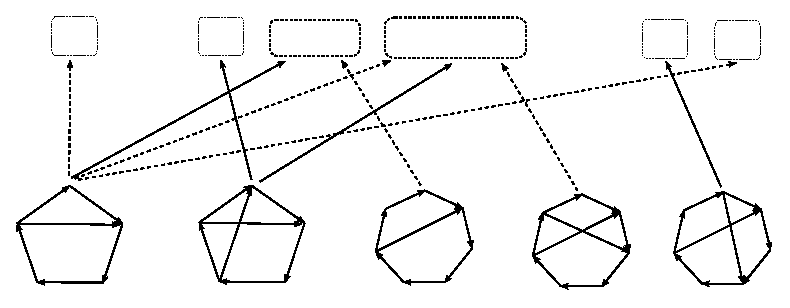
\includegraphics[width=12cm]{relation.eps}
\unitlength 0.86mm
\begin{picture}(1,1)(2,0)
\put(-132,45){\Large{$\mathrsfs{C}_n$}}
\put(-106,45){\Large{$\mathrsfs{D'}_n$}}
\put(-92,45){\Large{$\mathrsfs{W}_n$}}
\put(-84,45){\Large{$\mathrsfs{F}_n$}}
\put(-71,45){\Large{$\mathrsfs{E}_n$}}
\put(-64,45){\Large{$\mathrsfs{D''}_n$}}
\put(-54,45){\Large{$\mathrsfs{B}_n$}}
\put(-23,45){\Large{$\mathrsfs{G}_n$}}
\put(-10,45){\Large{$\mathrsfs{H}_n$}}
\put(-118, 47){\Large{$\ldots$}}
\put(-38, 47){\Large{$\ldots$}}
\end{picture}
\caption{Связь графов и автоматов}
\label{fig:relation}
\end{center}
\end{figure}

Приведем в заключении схему наших построений в виде рисунка~\ref{fig:relation}. Внизу представлены орграфы из теоремы~\ref{dulmage}(все,
кроме одного с экспонентой $n^2 - 3n + 2$). Прямая линия обозначает, что указанная серия получена с 
помощью раскрашивания, а пунктирная обозначает распетление.


\section{Эксперименты}
\label{experiments}
В этом разделе мы кратко изложим суть наших вычеслительных экспериментов.
Напомним, что детерминированный автомат $\mathrsfs{A}=\langle Q,\Sigma,\delta\rangle$ называется
\emph{достижимым}, если существует состояние $q_0\in Q$, из которого произвольное состояние 
$q\in Q$ достижимо, то есть, $q=\delta(q_0,w)$ для некоторого $w\in\Sigma^*$. В общем случае,
синхронизируемый автомат может не быть достижимым. Тем не менее, хорошо известно,
что при рассмотрении гипотезы Черни мы можем ограничиться рассмотрением сильно-связных автоматов,
поскольку справедливость в данном классе довольно легко влечет справедливость в общем
случае~\cite{Pi78}. Ясно, что всякий сильно-связный ДКА достижим.


%Here we briefly describe the settings of our experiments. Recall that a DFA
%$\mathrsfs{A}=\langle Q,\Sigma,\delta\rangle$ is said to be \emph{initially-connected}
%if there exists a state $q_0\in Q$ from which every state $q\in Q$ is reachable,
%that is, $q=\delta(q_0,w)$ for some $w\in\Sigma^*$. In general a \san\ need not
%be initially-connected. However, it is well known that when studying the \v{C}ern\'{y}
%conjecture, we may restrict ourselves to DFA whose underlying digraphs are strongly
%connected because the validity of the conjecture can be easily reduced to this case
%(see \cite{Pi78} for example). Clearly, DFA with strongly connected underlying digraphs
%are initially-connected.

Мы использовали удобное строковое представление достижимых ДКА, предложенное
в~\cite{AMR}, для порождения всех таких автоматов на двух буквах до 9 состояний
включительно. Всякий достижимый автомат был проверен на синхронизируемость, а
затем, вычислялась его граница синхронизации. В ходе проверок использовались
стандартные алгоритмы (смотрите~\cite{Sa05,Vo08}) реализованные на C.

%We used a convenient string representation of initially-connected DFA (ICDFA)
%developed in~\cite{AMR} to generate all such DFA with up to 9 states and 2 input
%letters. Each ICDFA was tested for synchronizability and then for each \san\
%its reset length was calculated. For these tasks, we implemented standard
%algorithms (see~\cite{Sa05,Vo08}) in C.

Основной трудностью таких вычислительных экспериментов является то, что количество
автоматов очень быстро растет с ростом числа состояний в них. Например, для 9 состояний
и всего двух входных букв существует уже более 700 миллионов достижимых автоматов.
Однако, наша вычислительная задача может быть легко распараллелена. А именно,
один узел порождал и распределял небольшие подмножества всех достижимых автоматов, а остальные
узлы проводили вычисления на получаемых подмножествах. Для реализации данного процесса
мы использовали известную библиотеку MPI. Вычисления, организованные указанным способом,
заняли меньше суток на довольно скромном кластере.


%The main difficulty that had to be overcome is that the number of ICDFA dramatically
%grows with the number of states. (For 9 states, there are about 700 billions
%ICDFA with 2 input letters.) The problem, however, can be efficiently parallelized.
%For this, a dedicated processor was programmed to generate ICDFA in portions (slices
%in terminology of~\cite{AMR}) that were fed to other processors for synchronization
%tests etc. The management program was written in C with MPI. Calculations organized
%this way took less than a day of running a small size computer grid based on a number
%of AMD Opteron 2.6 GHz processors.

Все найденные медленно-синхронизируемые автоматы были перепроверены с помощью
пакета TESTAS, разработанного Трахтманом~\cite{Tr06}.


%All slowly synchronizing automata that we found were double-checked by running on
%them the package TESTAS developed by Trahtman~\cite{Tr06}.

\begin{figure}[h]
\begin{center}
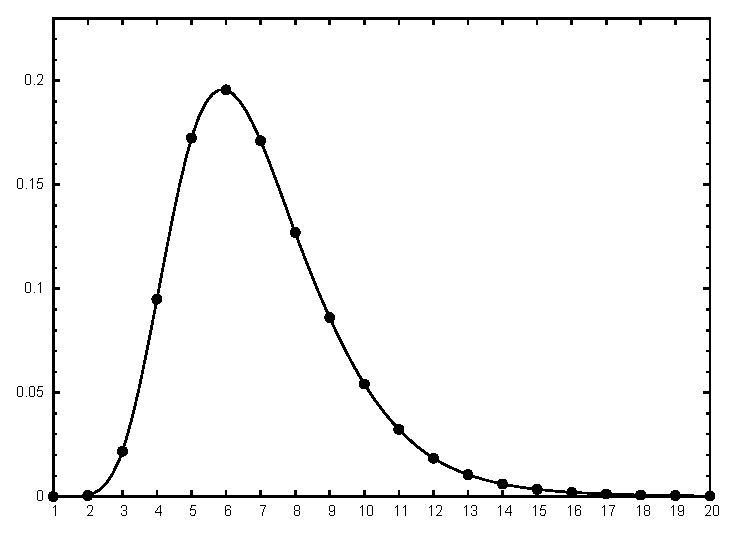
\includegraphics[width=10cm]{stat.eps}
\caption{Распределение двухбуквенных автоматов с 9 состояниями по границе синхронизации}
\label{fig:stat}
\end{center}
\end{figure}

Дополнительным результатом обширного вычислительного эксперимента является большой массив 
статистических данных. Представим собранные данные для достижимых синхронизируемых автоматов 
с двумя буквами и 9 состояниями на рисунке~\ref{fig:stat}. По горизонтальной оси отложена 
величина границы синхронизации, а по вертикальной оси -- доля синхронизируемых автоматов.
Жирная точка на рис.~\ref{fig:stat} с координатами $(x,y)$ означает, что доля $y$ синхронизируемых
автоматов обладает границей синхронизации $x$. Линия, соединяющая точки, представлена для
удобства восприятия. Напомним, что в данном случае, наибольшей достижимой границей
синхронизации является $64$. Видно, что большинство автоматов обладают сравнительно небольшим
синхронизирующим словом. А именно, почти все автоматы обладают синхронизирующим словом
не превосходящим $2n$. Это обстоятельсто хорошо согласуется с другими независимыми 
исследованиями~\cite{Tr11, ST}.

Нами также были построены аналогичные графики для достижимых двухбуквенных автоматов с 15 и 20
состояниями, основываясь на случайной выборке. Поведение их аналогично графику~\ref{fig:stat},
поэтому мы не будем их приводить.

\section{Заключение}
Нами предложен способ получения множества синхронизируемых автоматов с достаточно большой
границей синхронизации опираясь на известные результаты для экспонент примитивных графов.
Естественно возникает следующий вопрос: насколько указанный подход является универсальным?
Если указанные идеи окажутся хорошо применимы к различным классам автоматов, то это будет
свидетельствовать об исключительной связи между границами синхронизации и экспонентами.
Такая связь может послужить отправной точкой в попытке показать сраведливость гипотезы
Черни.

К несчастью, данные идеи несостоятельны. Попытка применить наш подход к классу эйлеровых 
автоматов была произведена в работе~\cite{Gu11}. Оказалось, что следуя нашему подходу,
можно добиться нижней оценки порядка $\frac{n^2}{4}$ на максимум границ синхронизации
среди эйлеровых автоматов с $n$ состояниями. Если же обобщить понятие экспоненты, то
можно достичь нижней оценки порядка $\frac{n^2}{2}$. Таким образом, можно искать
идею нового подхода к гипотезе Черни анализируя предложенные обобщения. Авторы надеются,
что исследование связанных понятий приведет к подтверждению этой интересной гипотезы.

\begin{thebibliography}{99}
\bibitem{AGW}
Adler, R.L., Goodwyn, L.W., Weiss, B.: Equivalence of topological Markov shifts.
Israel J. Math. 27, 49--63 (1977)

\bibitem{AS09}
Almeida, J.; Steinberg, B.: Matrix mortality and the \v{C}ern\'{y}--Pin
conjecture. In:  Diekert, V.; Nowotka, D. (eds.), Developments in
Language Theory, Lect.\ Notes Comput.\ Sci., vol.\,5583, pp. 67--80.
Springer, Heidelberg (2009)

\bibitem{AMR}
Almeida, M.; Moreira, N.; Reis, R.: Enumeration and generation with a string
automata representation. Theor.\ Comput.\ Sci. 387, 93--102 (2007)

\bibitem{AVZ}
Ananichev, D.S., Volkov, M.V., Zaks, Yu.I.: Synchronizing automata
with a letter of deficiency 2. Theor.\ Comput.\ Sci. 376, 30--41 (2007)

\bibitem{Br}
Brualdi R., Ryser H.: Combinatorial Matrix Theory. Cambridge University Press (1991).

\bibitem{Ce64}
\v{C}ern\'{y}, J.: Pozn\'{a}mka k homog\'{e}nnym eksperimentom s
kone\v{c}n\'{y}mi automatami. Matematicko-fyzikalny \v{C}asopis
Slovensk.\ Akad.\ Vied 14(3) 208--216 (1964) (in Slovak)

\bibitem{Du98}
Dubuc, L.: Sur les automates circulaires et la conjecture de
\v{C}ern\'y. RAIRO Inform.\ Th\'eor.\ Appl. 32, 21--34 (1998) (in
French)

\bibitem{DM62}
Dulmage, A.L., Mendelsohn, N.S.: The exponent of a primitive matrix.
Can.\ Math.\ Bull. 5, 241--244 (1962)

\bibitem{DM64}
Dulmage, A.L., Mendelsohn, N.S.: Gaps in the exponent set of primitive
matrices. Ill.\ J. Math. 8, 642--656 (1964)

\bibitem{Ep90}
Eppstein, D.: Reset sequences for monotonic automata. SIAM J.
Comput. 19, 500--510 (1990)

\bibitem{Gu11}
Gusev V.V.: Lower Bounds for the Length of Reset Words in Eulerian Automata, RP 2011,
Lect.\ Notes Comput.\ Sci., vol.\,6945, pp.\,180--190 (2011).

\bibitem{Hi88}
Higgins, P.M.: The range order of a product of $i$ transformations
from a finite full transformation semigroup, Semigroup Forum 37, 31--36
(1988)

\bibitem{Ka03}
Kari, J.: Synchronizing finite automata on Eulerian digraphs.
Theoret.\ Comput.\ Sci. 295, 223--232 (2003)

\bibitem{Pi78}
Pin, J.-E.: Le probl\`eme de la synchronization et la conjecture de
\v{C}ern\'y. Th\`ese de 3\`eme cycle. Universit\'e de Paris 6 (1978) (in
French)

\bibitem{Pi83}
Pin, J.-E.: On two combinatorial problems arising from automata
theory. Ann.\ Discrete Math. 17, 535--548 (1983)

\bibitem{RaAl05}
Ram\'{\i}rez Alfons\'{\i}n, J.L.: The diophantine Frobenius problem.
Oxford University Press (2005)

\bibitem{Sa05}
Sandberg, S.: Homing and synchronizing sequences. In: Broy, M.
et~al. (eds.), Model-Based Testing of Reactive Systems. Lect.\
Notes Comput.\ Sci., vol.\,3472, pp.\,5--33. Springer, Heidelberg
(2005)

\bibitem{ST}
Skvortsov E., Tipikin E.: Experimental Study of the Shortest 
Reset Word of Random Automata, CIAA 2011, Lect.\
Notes Comput.\ Sci., vol.\,6807, pp.\,290--298 (2011).

\bibitem{SZ}
Skvortsov E., Zaks Yu.: Synchronizing random automata. Submitted;
proceedings version in: Rigo, M. (ed.), AutoMathA 2009, Universit\'e
de Li\`ege (2009)

\bibitem{Tr06}
Trahtman, A.N.: An efficient algorithm finds noticeable trends
and examples concerning the \v{C}ern\'y conjecture. In:
Kr\'alovi\v{c}, R.; Urzyczyn, P. (eds.), Mathematical Foundations
of Computer Science. Lect.\ Notes Comput.\ Sci., vol.\,4162, pp.\,789--800
Springer, Heidelberg (2006)

\bibitem{Tr06a}
Trahtman, A.N.: Notable trends concerning the synchronization
of graphs and automata. Electr.\ Notes Discrete Math. 25, 173--175 (2006)

\bibitem{Tr07}
Trahtman, A.N.: The \v{C}ern\'y conjecture for aperiodic automata.
Discrete Math.\ Theor.\ Comput.\ Sci. 9(2), 3--10 (2007)

\bibitem{Tr08}
Trahtman, A.N.: Some aspects of synchronization of DFA. J. Comput.\ Sci.\
Technol. 23, 719--727 (2008)

\bibitem{Tr09}
Trahtman, A.N.: The Road Coloring Problem. Israel J. Math.
\textbf{172}, 51--60 (2009)

\bibitem{Tr11}
Trahtman A.N.: Modifying the Upper Bound on the Length of Minimal Synchronizing
Word. Lect. Notes in Comp. Sci, 173--180, 6914 (2011)

\bibitem{Vo08}
Volkov, M.V.: Synchronizing automata and the \v{C}ern\'{y}
conjecture. In: Mart\'\i{}n-Vide, C.; Otto, F.; Fernau, H. (eds.),
Languages and Automata: Theory and Applications. Lect.\ Notes
Comput.\ Sci., vol.\,5196, pp.\,11--27.  Springer, Heidelberg (2008)

\bibitem{Vo09}
Volkov, M.V.: Synchronizing automata preserving a chain of partial
orders. Theoret.\ Comput.\ Sci. 410, 2992--2998 (2009)

\bibitem{Wi50}
Wielandt, H.: Unzerlegbare, nicht negative Matrizen. Math.\ Z.
52, 642--648 (1950) (in German)
\end{thebibliography}


\end{document}
